% ||================================================================================================
% || Präambel
% ||================================================================================================

% |=================================================================================================
% | Layout
% |=================================================================================================
\documentclass[11pt,titlepage]{book}
% digital
% print
%\documentclass[12pt,titlepage]{book}
\usepackage{geometry}
\geometry{
  left=3cm,
  right=3cm,
  % print
  % bindingoffset=5mm
}

% |=================================================================================================
% | Fonts
% |=================================================================================================
\usepackage[onehalfspacing]{setspace}
\usepackage{dejavu} 
\usepackage{sectsty}
\allsectionsfont{\sffamily}
\usepackage[T1]{fontenc}
\usepackage[utf8]{inputenc} % direkte Einbgabe von Umlauten

% language stuff
\usepackage[german]{babel}

% miscellaneous
\usepackage{graphicx, subfigure}         % graphics
\graphicspath{{grafiken/}}
\usepackage{hhline}           % double lines in tables
\usepackage{amsfonts}         % real numbers etc.
\usepackage{amsmath}
\usepackage[rightcaption]{sidecap} % figure captions on the right (optional)
\usepackage{hyperref}         % for URLs
\usepackage{listings}         % for code samples
\usepackage{fancyhdr}         % for header line

\usepackage[backend=biber, style=authoryear, maxbibnames=99]{biblatex}
\addbibresource{literatur.bib}
\DeclareNameAlias{default}{family-given}
\DeclareNameAlias{sortname}{family-given}

\usepackage[german]{algorithm2e}
\RestyleAlgo{ruled}

\usepackage[german]{cleveref}

\usepackage{afterpage}

\newcommand\blankpage{
    \null
    \thispagestyle{empty}
    \addtocounter{page}{-1}
    \newpage
}
    
\usepackage{multirow, multicol, tabularx}
\usepackage{csquotes}

\usepackage{ifluatex}
\ifluatex
  \usepackage{pdftexcmds}
  \makeatletter
  \let\pdfstrcmp\pdf@strcmp
  \let\pdffilemoddate\pdf@filemoddate
  \makeatother
\fi
\usepackage{svg}

\hyphenation{Data-Frame Data-Frames}

\title{Arbeit}
\author{Alexander Martin}
\date{August 2021}
\begin{document}


\let\origdoublepage\cleardoublepage
\newcommand{\clearemptydoublepage}{%
    \clearpage
    {\pagestyle{empty}\origdoublepage}%
}

\pagestyle{empty}
\begin{titlepage}
  \begin{center}
    {\Large\bf Entwurf und Implementierung einer generischen Ingestion-Schnittstelle mit Versionierung für Data-Lake-Systeme}\\[2cm]

    {\bf Masterarbeit}\\
    zur Erlangung des Grades {\em Master of Science}\\[1cm]

    an der\\
    Hochschule Niederrhein\\
    Fachbereich Elektrotechnik und Informatik\\
    Studiengang {\em Informatik}\\[2cm]

    vorgelegt von\\
    Alexander Martin\\
    1018332\\[3cm]
    Datum: \today\\[2cm]

    Prüfer: Prof.~Dr.~rer.~nat.~Christoph Quix\\
    Zweitprüfer: Sayed Hoseini,~M.Sc.

  \end{center}
\end{titlepage}
\afterpage{\blankpage}
\section*{Eidesstattliche Erklärung}

\begin{tabbing}
  Name: \hspace{4em}\= Alexander Martin\\
  Matrikelnr.: \> 1018332\\
  Titel: \> Entwurf und Implementierung einer generischen \\ 
         \> Ingestion-Schnittstelle mit Versionierung für Data-Lake-Systeme
\end{tabbing}

Ich versichere durch meine Unterschrift, dass die vorliegende
Arbeit ausschließlich von mir verfasst wurde.
Es wurden keine anderen als die von mir angegebenen Quellen und Hilfsmittel
benutzt.

Die Arbeit besteht aus \underline{\hspace{3em}} Seiten.

\vspace{8ex}
\begin{tabbing}
  \underline{\hspace{14em}} \hspace{3em}\= \underline{\hspace{14em}} \\
  Ort, Datum \> Unterschrift
\end{tabbing}
\afterpage{\blankpage}
\section*{Zusammenfassung}
asd
\section*{Abstract}
asd
\let\cleardoublepage\clearemptydoublepage

% Kopf- und Fußzeile
\fancyhead{} % clear all header fields
\fancyhead[RO,LE]{\leftmark}
\setlength{\headheight}{15pt}
\pagestyle{fancy}
\tableofcontents
\chapter{Einleitung}

\section{Die Motivation}
In der heutigen Zeit spielen Daten in der Welt eine immer größere Rolle.
In \textit{Rethink Data Report 2020} \textcite{rethink_data_2020} wurde eine Studie durchgeführt, die eine Steigerung von 42\% der Menge an anfallenden Daten pro Jahr prognostiziert.
Dies wird unter anderem auf den vermehrten Einsatz von IoT-Geräten, immer ausführlicheres Analysieren von Daten und die einfacher werdende Anwendung von Cloud-Speichern zurückgeführt.
Dabei besteht die Herausforderung, Daten in verschiedensten Formaten in großen Mengen zu verwalten und zu verwenden.

Ein Lösungansatz für dieses Problem sind Data-Lake-Systeme.
Data-Lake-Systeme sind zentrale Datenspeicher, die strukturierte, semi- und unstrukturierte Daten in ihrem Rohformat speichern.
Mit Hilfe von Metadaten bietet ein Datalake Schnittstellen zur Datenanalyse und -abfrage.
Dabei funktioniert das System nach dem Schema-On-Read oder auch ELT (Extrahieren Laden Transformieren) Prinzip.
Das bedeutet, dass die Daten wie bereits erwähnt im Rohformat im Data Lake gespeichert werden und erst nach dem Laden ein entsprechendes Schema angewendet wird.

Es gibt bereits viele Anbieter, die fertige Data-Lake-Systeme anbieten.
Dabei ist jedoch ein Nachteil, dass sie häufig nur in der (Cloud-)Infrastruktur des Anbieters (z.B. Microsoft Azure\footnote{https://azure.microsoft.com/}, Amazon Web Services\footnote{https://aws.amazon.com/}) verfügbar sind und sich ihrere Architektur nach diesen Diensten richtet.
Daher wird in dieser Arbeit eine Schnittstelle für die Ingestion, also das Laden der Daten in das Data-Lake-System, entwickelt, die in einem platform unabhängigen Data-Lake-System Anwendung finden soll.

\section{Der Aufbau}
Am Anfang wird auf die Ziele eigengangen, die Schnittstelle erreichen soll.
Aus diesen Zielen werden dann konkrete Anforderungen an die Entwicklung abgeleitet.
Im zweiten Kapitel wird das System der Schnittstelle entwickelt, ohne dabei auf konkrete Details, wie zum Beispiel Programmiersprachen, einzugehen.
Hier geht es mehr um die Architektur und das Design, das benötigt wird um alle Anforderunegn abzudecken.
Danach wird die Umsetzung beschrieben.
Hierbei spielt vorallem das bereits exisitierende Data-Lake-System, in dem die Ingestion-Schnittstelle integriert werden soll, eine große Rolle.
Zum Schluss wird die Ingestion-Schnittstelle evaluiert und ein Ausblick auf mögliche weitere Arbeiten gegeben.

\section{Das Existierende System}
In dem Masterprojekt \textit{Development of a Data Lake System} \parencite{datalake_proj} an der Hochschule Niederrhein wurde bereits eine Data-Lake-System-Prototyp entwickelt.
Das System ist eine monolithische Client-Server-Anwendung.
Es besteht aus einer REST-API, die zur Interaktion mit dem Data-Lake-System verwendet wird und einem Web-Frontend.
Außerdem können durch einfach Anpassungen der Server-Anwendung beliebige Datenspeicher in das Data-Lake-System integriert werden.

Als Basis wird \textit{Apache Spark}\footnote{https://spark.apache.org/} verwendet.
\textit{Apache Spark} ist eine Plattform, um Analyse auf großen Datenmengen aus zu führen.
Außerdem gibt es Schnittstellen für \textit{Scala, Java und Python} und es wird auch die Verarbeitung von Datenströmen und maschinelles Lernen unterstützt \parencite{spark}.

Der Server ist in \textit{Python} geschrieben und verwendet das Framework \textit{Flask}\footnote{https://palletsprojects.com/p/flask/} um eine REST-API bereitzustellen, über die mit dem Data Lake interagiert werden kann.
Dabei werden über die API \textit{JSON}-Objekte ausgetauscht, so dass die API client-unabhängig verwendet werden kann.
Der Client des Projekts ist eine Webanwendung, die mit \textit{Angular}\footnote{https://angular.io/} umgesetzt wurde.

\section{Verwandte Arbeiten}

\subsection{Techniken}

\subsubsection{Apache Spark}

\subsubsection{Apache Kafka}

\textit{Apache Kafka} ist ein verteiltes Event-Streaming-System, dass nach dem Publish-Subscribe-Muster funktioniert.
Events können von Produzenten in das System veröffentlicht werden und Konsumenten können diese Events abonnieren.
Das ganze läuft dabei in Echtzeit ab.
Durch seine Verteilung kann \textit{Kafka} den Ausfall einzelner Server ausgleichen.
Außerdem können Ströme von Events für einen beliebigen Zeitraum abgespeichert werden.

\textit{Kafka} besteht aus einem Cluster von Servern und verschiedenen Clients.
Es gibt zwei Arten von Servern.
Einige bilde die Speicherebene von \textit{Kafka} und werden Broaker genannt.
Die anderen verwenden \textbf{Kafka Connect}\footnote{https://kafka.apache.org/documentation/\#connect} um existierende Systeme, zum Beispiel eine Datenbank, in das Kafka Cluster zu integrieren.
Anwendungen, die entweder Events produzieren oder konsumieren sind die Clients.

In diesem System repräsentiert ein Event den Fakt, dass etwas "`passiert"' ist und besteht aus einem Schlüssel, einem Wert, einem Zeitstempel und optionalen Metadaten.
Dabei werden die Werte nicht interpretiert sonder einfach als Block versendet und können so beliebige Struktur haben.
Events werden in sogenannte Topics unterteilt.
Es kann immer mehrere Produzenten oder Konsumenten auf einer Topic geben.
Events in einer Topic können mehrfach gelesen werden und werden nicht nach dem Konsumieren gelöscht.
Es kann aber für jede Topic einzeln eine Dauer festgelegt werden, nach der die Events verworfen werden.
Um eine Topic fehlertolerant zu machen, kann diese repliziert werden.

Topics werden in Partitionen über verschiedene Broaker aufgeteilt, so dass das ganze System gut skalierbar wird.
Ein Produzenten kann zum Beispiel Events auf mehreren Brokern gleichzeitig veröffentlichen.
Wenn ein Event in einer Topic veröffentlicht wird, wird dieses an eine der Partitionen angehängt.
Events, die den gleichen Schlüssel haben werden immer der gleichen Partition zugeordnet und Events einer Partition kommen garantiert in der Reihenfolge des Schreibens bei dem Konsumenten der Partition an \parencite{kafka-docs}.

\textit{Apache Kafka} wird im Big Data Bereich weit verbreitet um Datenströme zu verarbeiten.
Daher macht es Sinn, \textit{Kafka} auch in dieses Data Lake System zu integrieren und darin bereit zu stellen.
Außerdem kann es auch für die Kommunikation zwischen den verschiedenen Microservices verwendet werden.

\subsection{Hadoop Distributed File System}

Als Speicher wird das \textit{Hadoop Distributed File System (HDFS)} verwendet.
Das \textit{HDFS} ist ein verteiltes, auf große Dateien ausgelegtes Dateisystem.
Ein \textit{HDFS} Cluster besteht aus einem Namenode und mehreren Datanodes.

Der Namenode verwaltet den Baum des Dateisystems und kontrolliert den Zugriff durch Clients.
Zusätzlich führt er Operation auf dem Dateisystem aus.
Dazu zählen das Öffnen, Schließen oder Umbenennen von Dateien oder Ordnern.
Die Dateien selbst werden in Blöcke aufgeteilt auf den Datanodes gespeichert.
Diese sind auch dafür verantwortlich, Lese- und Schreibanfragen zu bedienen und verwalten die Erstellung, Löschung und Replikation unter Anleitung des Namenodes \parencite{hdfs}.

Das \textit{HDFS} ist ebenfalls eine weit verbreitete Technik im Big Data Bereich und eignet sich auch hier, durch die Auslegung auf große Dateien, sehr gut um die Quelldateien der Datenquellen abzulegen.
Außerdem sind Dateien auf allen Servern verfügbar, da es sowohl eine REST-Schnittstelle als auch Unterstützung in \textit{Apache Spark} gibt.

\chapter{Grundlagen und Verwandte Arbeiten}

Dieses Kapitel befasst sich mit den technischen Grundlagen dieser Arbeit und verwandten Arbeiten.
Unter den technischen Grundlagen werden zunächst Rahmenwerke erklärt, die im Laufe dieser Arbeit eingesetzt werden.
% ab hier eventuell nochmal bearbeiten
Danach folgt eine genauere Erklärung von Data Lakes.
Zum Schluss wird auf das Change-Data-Capture (deutsch: Änderungserfassung) eingegangen.
Das ist nicht direkt Teil der Entwicklung in dieser Arbeit, spielt aber im Anwendungsbereich eine große Rolle.

\section{Technische Grundlagen}
\subsection{Hadoop}

Hadoop\footnote{https://hadoop.apache.org/} ist ein Projekt von Apache für die verteilte Datenverarbeitung auf einem Cluster.
Die Verarbeitung basiert auf  Map-Reduce \parencite{mapred}, einem Programmier-Modell, bei dem Daten in Form von Schlüssel-Wert-Paaren verarbeitet werden.
Grob beschrieben, besteht es aus zwei Funktionen.
Die erste ist die Map-Funktion, bei der aus Daten eine Zwischensammlung von Schlüssel-Wert-Paaren erzeugt wird.
Danach werden diese nach den Schlüsseln sortiert und die Reduce-Funktion, zum Zusammenfassen der Paare ausgeführt.
Ein Hadoop-Cluster enthält zwei wichtige Komponenten.
YARN \parencite{yarn} wird für das Ressourcen-Management benutzt.
Die zweite Komponente, das HDFS, ist ein verteiltes und fehlertolerantes Dateisystem, welches ursprünglich für Hadoop entwickelt wurde.
Für dieses Projekt ist nur das HDFS relevant und wird deswegen näher erläutert.

Das HDFS wurde entwickelt, um auf Hardware mit geringen Kosten zu laufen und große Datenmengen zu verarbeiten.
Dateien können von einem Gigabyte bis mehrere Terabyte groß sein.
Die Fehlertoleranz wird dabei durch die Möglichkeit der Replikation mit einem beliebigen Faktor gegeben.

Das Dateisystem ist ähnlich zu anderen bekannten Dateisystemen aufgebaut.
Dateien und Ordner können im Namensraum hierarchisch organisiert werden.
Es unterstützt jedoch keine Zugriffsberechtigung oder Hard- und Soft-Links.
Um einfach und effektiv kohärent zu bleiben, werden Dateien nur einmal geschrieben, können aber mehrfach gelesen werden.
Dateien werden zur Speicherung in einzelne Blöcke aufgeteilt.
Dabei sind für eine Datei alle Blöcke, bis auf den letzten, gleich groß.

\begin{figure}
    \centering
    \includegraphics[width=\textwidth]{Grafiken/Grundlagen/HDFS.pdf}
    \caption[HDFS-Architektur]{HDFS-Architektur\footnotemark}
    \label{fig:hdfs-cluster}
\end{figure}
\footnotetext{Nach https://hadoop.apache.org/docs/r1.2.1/images/hdfsarchitecture.gif, Zugriff: 29.12.2021}

Ein HDFS-Cluster (\cref{fig:hdfs-cluster}) funktioniert nach dem Master-Worker-Prinzip und besteht aus einem NameNode und vielen DataNodes.
Der NameNode übernimmt die Verwaltung des Namensraums und die Verteilung der einzelnen Blöcke einer Datei.
Er reguliert dazu noch den Zugriff durch Clients und führt Operationen auf dem Dateisystem, wie das Öffnen, Schließen oder Umbenennen von Ordnern und Dateien aus.
Die DataNodes speichern die einzelnen Blöcke der Dateien.
Auf Anweisung des NameNode werden Blöcke erstellt, gelöscht oder repliziert.
Außerdem bearbeiten sie Anfragen zum Lesen und Schreiben von Dateien \parencite{hdfs}.

% Parquet
Mit Apache Parquet steht ein Format zur Verfügung, mit dem Daten im HDFS effizient gespeichert werden können.
Parquet ist ein spalten-orientiertes Speicherformat, das auch die Kompression und Kodierung der Daten unterstützt.
Über einen Algorithmus zur Zerlegung von Verschachtelung ist auch das Speichern von semistrukturierten Daten möglich \parencite{parquet}.

\subsection{Apache Spark}
\label{sec:spark}

Apache Spark ist eine Datenverabeitungs-Engine für die effiziente, verteilte Verarbeitung von Big Data.
Das Ziel bei der Entwicklung von Apache Spark war es, ein einheitliches Rahmenwerk für Big-Data-Prozesse zu schaffen.
Das Problem war, dass die bis dahin verbreitetste Lösung Hadoop keine einheitliche Abfragesprache und kein einheitliches Datenmodell hat.
Durch Spark ist das Arbeiten mit zum Beispiel SQL, Datenströmen, maschinellem Lernen oder Graph-Daten möglich.
Es gibt viele Bibliotheken für die Verwendung verschiedener Datenquellen in Spark.
Durch ihre Optimierung erreichen diese eine ähnliche Performance wie manuell dafür implementierte Big-Data-Prozesse.
Spark kann entweder lokal auf einem Computer oder auf einem Spark-Cluster nach dem Master-Worker-Modell ausgeführt werden.

Ein Kernprinzip ist die Abstraktion der Daten in RDDs (Resilient Distributed Datasets, deutsch: Resiliente Verteilte Datensätze).
RDDs sind fehlertolerante Sammlungen von Objekten, die auf die Worker-Instanzen verteilt und parallel bearbeitet werden können.
Diese werden flüchtig im Hauptspeicher gehalten, können aber für spätere schnellere Zugriffe zwischengespeichert (persistiert) werden.
Die Erstellung und Bearbeitung von RDDs geschieht über sogenannte Transformationen.
Die Transformationen werden in einem Herkunftsgraphen gespeichert, wodurch eine Wiederherstellung bei Fehlern an jedem Punkt möglich ist.

Für die Verarbeitung von strukturierten oder semistrukturierten Daten gibt es zusätzlich die eigene Abfragesprache SparkSQL, die sich stark an SQL orientiert.
Es gibt Bibliotheken für die Sprachen Scala, Java, Python und R.
Auf den RDDs gibt es noch eine weitere Abstraktionsebene, die DataFrames.
Mit DataFrames, die eine Sammlung RDDs von Datensätzen mit einem bekannten Schema sind, kann eine API benutzt werden, bei der die Bearbeitung der Daten über Funktionsaufrufe statt SparkSQL möglich ist \parencite{spark}.

Die Interaktion mit einem Spark-Cluster kann über eine interaktive Shell oder einen, in einer der unterstützen Sprachen programmierten, Job geschehen.
Informationen über die Anwendung werden im SparkContext gespeichert.
Beim Lesen und Schreiben wird das Format der Daten angegeben.
Spark unterstützt standardmäßig einige Formate, aber durch die Konfiguration mit zusätzlichen Bibliotheken im SparkContext, kann die Unterstützung weiterer Formate hinzugefügt werden.
Von den verwendeten Bibliotheken und dem Format sind auch die Optionen abhängig, die beim Lesen und Schreiben gesetzt werden müssen.
Die Optionen sind immer Schlüssel-Wert-Paare und enthalten zum Beispiel Verbindungsinformationen zu einer Datenbank oder einem Dateispeicherort \parencite{spark-website}.

\subsection{Apache Kafka}
\label{sec:kafka}

Apache Kafka ist ein verteiltes Event-Streaming-System.
Die Vermittlung der auftretenden Events läuft in Echtzeit ab.
Kafka basiert auf dem nach dem Publish-Subscribe-Modell.
Events können von Produzenten veröffentlicht werden und Konsumenten können auf diese Events abonnieren.
Durch die Verteilung in einem Cluster kann Kafka den Ausfall einzelner Server ausgleichen.
Zusätzlich können Ströme von Events für einen beliebigen Zeitraum gespeichert werden.

Kafka besteht aus einem Cluster von Servern und verschiedenen Clients.
Es gibt zwei Arten von Servern.
Die sogenannten Broaker sind für die Verteilung und Verwaltung von Events zuständig.
Andere verwenden Server Kafka Connect\footnote{https://kafka.apache.org/documentation/\#connect} um existierende Systeme, wie zum Beispiel ein Datenbank-System, in das Kafka-Cluster zu integrieren.
Die Clients sind Anwendungen, die entweder Events produzieren oder konsumieren.

In diesem System repräsentiert ein Event den Fakt, dass etwas "`passiert"' ist und besteht aus einem Schlüssel, einem Wert, einem Zeitstempel und optionalen Metadaten.
Dabei werden die Werte nicht interpretiert sonder einfach als Byte-Block versendet und können so beliebige Struktur haben.
Events werden in sogenannte Topics unterteilt.
Es kann immer mehrere Produzenten oder Konsumenten auf einem Topic geben.
Events in einem Topic können mehrfach gelesen werden und werden nicht nach dem Konsumieren gelöscht.
Es kann aber für jedes Topic eine Dauer festgelegt werden, nach der die Events verworfen werden.
Um ein Topic fehlertolerant zu machen, kann dieses repliziert werden.

Topics werden in Partitionen über verschiedene Broker aufgeteilt, so dass das ganze System gut skalierbar wird.
Ein Produzenten kann zum Beispiel Events auf mehreren Brokern gleichzeitig veröffentlichen.
Wenn ein Event in einem Topic veröffentlicht wird, wird dieses an eine der Partitionen angehängt.
Events, die den gleichen Schlüssel haben werden immer der gleichen Partition zugeordnet und Events einer Partition kommen garantiert in der Reihenfolge des Schreibens bei dem Konsumenten der Partition an \parencite{kafka-docs}.

Konsumenten können auch in Gruppen zusammengefasst werden.
Innerhalb einer Gruppe werden Events eines Topics innerhalb der Mitglieder, die dieses Topic abonniert haben, aufgeteilt.
Diese Funktion kann zum Beispiel für den Lastausgleich verwendet werden.

\section{Data Lake}
In der Einleitung (\cref{sec:einleitung-datalake}) wurde der Data Lake als Lösung für die Probleme der Datenerfassung im Big-Data-Bereich bereits kurz beschrieben.
In diesem Abschnitt wird noch einmal genauer auf Data-Lake-Systeme, deren Definition, Architektur und existierende Systeme eingegangen.

\subsection{Definition eines Data Lake}
Neben der Definition, die in der Einleitung gegeben wird, wurde von \textcite{sawadogo2021data} eine detailliertere Definition für Data Lakes aufgestellt.
Hiernach sind Data-Lake-Systeme ein skalierbarer Speicher für Daten jeden Typs.
Die Daten werden im Rohformat gespeichert und hauptsächlich durch Datenspezialisten, wie Statistiker oder Analysten, für die Extraktion von Wissen verwendet.
Ein Data Lake hat dabei die folgenden Eigenschaften: \begin{enumerate}
    \item ein Metadaten-Katalog, um die Datenqualität sicher zu stellen,
    \item Regeln und Werkzeuge für die Data Governance,
    \item Zugänglichkeit zu den Daten für verschiedene Arten von Benutzern,
    \item die Integration von Daten jeden Typs,
    \item sowohl eine logische als auch eine physische Gliederung und
    \item die Skalierbarkeit von Speicher und Verarbeitung.
\end{enumerate}

\subsection{Architekturen für Data Lakes}
Von \textcite{inmon2016data} wird das System in sogenannten Ponds (Teiche) strukturiert.
Jeder Pond ist mit einem spezialisierten Speichersystem verknüpft und beinhaltet Daten eines bestimmten Typs.
Einige Ponds führen zudem weitere Verarbeitungen der Daten, wie Aufbereitung oder Analysen aus.
Inmon hat eine Architektur aus fünf Ponds aufgestellt (\cref{fig:datalake-ponds}).
\begin{enumerate}
    \item Daten werden im \emph{Raw Data Pond} im Rohformat gespeichert und fließen von dort aus in andere Ponds.
          Dieser dient also als Eintrittspunkt in das System für neue Daten.
          Nach dem Verlassen des Pond werden die Daten aus diesem gelöscht.
    \item Der \emph{Analog Data Pond} enthält analoge Daten, meist von IoT-Geräten.
          Diese werden hier auf ein aussagekräftiges und verwaltbares Volumen reduziert und umstrukturiert.
    \item In den \emph{Application Data Pond} kommen Daten, die von Software-Anwendungen erzeugt wurden.
          Diese sind häufig strukturierte Daten aus relationalen Daten\-bank-Systemen.
          Sie werden für Analysen integriert und aufbereitet.
    \item Der \emph{Textual Data Pond} enthält unstrukturierte Daten und Prozesse, die deren Analyse erleichtern.
    \item Im \emph{Archival Data Pond} werden alle Daten gespeichert, die nicht mehr aktiv verwendet, aber eventuell in der Zukunft nochmal gebraucht werden.
\end{enumerate}
\begin{figure}
    \centering
    \includegraphics[width=.8\textwidth]{Grafiken/Grundlagen-Ponds.pdf}
    \caption{Ponds-Architektur \parencite[nach: ][S. 27]{inmon2016data}}
    \label{fig:datalake-ponds}
\end{figure}

Ein anderer Ansatz ist die Unterteilung des Data Lake in Zonen (\cref{fig:datalake-zones}).
Hier werden die Daten nach ihrem Verfeinerungsgrad in einer entsprechenden Zone abgelegt.
Dabei durchlaufen sie die einzelnen Zonen hintereinander.
Die Anzahl der Zonen und deren Verfeinerungsgrad ist dabei je nach Anwendung unterschiedlich \parencite{dl-zones}.

\begin{figure}
    \centering
    \includegraphics[width=.8\textwidth]{Grafiken/Grundlagen-Zones.pdf}
    \caption{Prinzip der Zonen-Architektur}
    \label{fig:datalake-zones}
\end{figure}

Eine speziellere Architektur ist die Lambda-Architektur, die für die verteilte Verarbeitung von Echtzeit- und Batch-Daten verwendet wird.
Eine Lambda-Architektur besteht aus drei Ebenen (Layers) \parencite{lambda-arch}: \begin{enumerate}
    \item Die \emph{Batch Layer} hat zwei Aufgaben.
          Die erste Aufgabe ist das verteilte Speichern von wachsenden Daten.
          Dafür kann zum Beispiel das HDFS verwendet werden.
          Als zweite Aufgabe werden Batch Views für die verteilten Daten vorberechnet, um Anfragen schneller beantworten zu können.
    \item In der \emph{Speed Layer} werden inkrementell Echtzeit-Views auf Daten verwaltet.
          Dadurch wird die Lücke gefüllt, die bei den Views in der Batch-Ebene entstehen können.
          Die Speed Layer enthält immer nur aktuelle Daten.
          Ältere Daten werden durch die Batch Layer aufgenommen.
    \item Die \emph{Serving Layer} enthält Indices über alle Batch Views um Anfragen mit geringer Latenz bearbeiten zu können. Sie ist dafür verantwortlich die Views aus der Batch und der Speed Layer zusammenzuführen um Echtzeitergebnisse über alle Daten bereit zu stellen.
\end{enumerate}

Nach \textcite{sawadogo2021data} können die Architekturen von Data-Lake-Systemen auch anders unterteilt werden.
Bei datenorientierten Architekturen wird der Data Lake in verschiedene Datenbereiche unterteilt.
Die funktionsorientierten Architekturen dagegen teilen das Data-Lake-System nach den Funktionen auf, die in ähnlichen Bereichen zusammengefasst werden.
Ein Beispiel ist die Architektur aus der Einleitung von \textcite{datalake_03}.
In hybriden Architekturen können auch beide Ansätze kombiniert werden.

\subsection{Data-Lake-Systeme und Rahmenwerke}
Es gibt bereits verschiedene Rahmenwerke oder Systeme für die Umsetzung eines Data Lake.
Nachfolgend wird eine Auswahl daraus vorgestellt.

\paragraph{CoreDB} CoreDB ist ein Service, der es erlaubt über eine einzige REST-API Daten und Metadaten in einem Data Lake zu organisieren, zu indizieren und abzufragen.
Es können sowohl relationale als auch NoSQL-Datenbanksysteme mit CoreDB verwendet werden.
Für die Suche in den Daten wird elastic\footnote{https://www.elastic.co/} verwendet.
Das Design von CoreDB unterstützt Funktionen für die Sicherheit und Zugriffskontrolle und die Verfolgung und Herkunft, um überwachende Metadaten sammeln zu können \parencite{coredb}.

\paragraph{Azure Data Lake} In dem Cloud-Angebot von Microsoft gibt es den Azure Data Lake\footnote{https://azure.microsoft.com/de-de/solutions/data-lake/}.
Hier werden viele Funktionen, die für den Aufbau eines Data Lake notwendig sind als Cloud-Lösung bereitgestellt.
Dazu gehören unter anderem Hadoop, Apache Spark und ein Speichersystem zum Speichern aller Daten.
Außerdem gibt es weitere Dienste zur Analyse oder Integration der Daten.

\paragraph{Kylo} Kylo\footnote{https://kylo.io/} ist ein Projekt für eine Data-Lake-Management-Plattform.
In dieser Plattform ist eine Ingestion-Komponente enthalten, die die Bereinigung und Validierung von Daten unterstützt.
Außerdem gibt es Funktionen für die Aufbereitung und Erkundung von Daten oder zur Systemüberwachung.
Zusätzlich ist Apache Nifi\footnote{https://nifi.apache.org/} zur Erstellung von Verarbeitungs-Pipelines integriert.
Die Entwicklung an Kylo wird seit über einem Jahr nicht mehr fortgeführt.

\paragraph{Hudi} Apache Hudi\footnote{https://hudi.apache.org/} ist eine Plattform, um selbst-verwaltete Data Lakes mit einer Optimierung für Datenstromverarbeitung aufzubauen.
Zu den Features von Hudi gehört zum Beispiel die Indizierung von Änderung und das Zurückgehen in den Daten zu einem bestimmten Zeitpunkt.
Hudi unterstützt sowohl inkrementelle Abfragen als auch Batch-Verarbeitung von Daten.

\paragraph{}
Bei diesen Systemen fehlen entweder eine ausführliche Metadatenpflege oder eine Datenversionierung, sie bilden nur einen bestimmten Teil eines Data Lake oder sind für spezielle Anwendungsfälle.
Daher wurde bisher kein geeignetes Data-Lake-System für die Anwendung am HIT gefunden

\subsection{Delta Lake}

Als eine Lösung für die Versionierung von Daten gibt es den Delta Lake.
Delta Lake ist eine extra Speicherebene, die auf dem HDFS oder einem Objektspeicher in der Cloud, wie Amazons S3, angewendet werden kann.
Das Ziel ist es, diesen Speichern ACID-Transaktionen, schnelles Arbeiten mit Metadaten der Tabelle und eine Versionierung der Daten hinzuzufügen.
Daten werden in sogenannten Delta-Tabellen mit Metadaten und Logs gespeichert.

Eine Delta-Tabelle wird zunächst durch ein Verzeichnis im Dateisystem dargestellt.
Die tatsächlichen Daten werden in diesem Verzeichnis als Parquet-Dateien abgelegt.
Dabei können die Daten auch noch in Unterverzeichnisse aufgeteilt werden, zum Beispiel für jedes Datum ein Verzeichnis.
Neben den Datenverzeichnissen gibt es in jeder Delta-Tabelle einen Ordner für die Logs in Form von JSON Dateien mit aufsteigender Nummerierung.
Metadaten werden sowohl innerhalb der Parquet- als auch in der Log-Dateien gespeichert.

Im Delta Lake wird ein Protokoll für den Zugriff verwendet, dass es mehreren Clients ermöglicht gleichzeitig lesen zu können, aber immer nur einem das Schreiben erlaubt.
Dabei werden beim Schreiben immer erst neue Datensätze, die zur Tabelle hinzugefügt werden sollen, in das Verzeichnis der Delta-Tabelle geschrieben.
Danach wird eine neue Log-Datei erstellt.

Beim Lesen werden die Log-Dateien als Grundlage verwendet um, daraus zusammen mit den gespeicherten Daten den Zustand der Tabelle an einem bestimmten Zeitpunkt zu erzeugen.
Standardmäßig wird beim Lesen immer die aktuellste Version verwendet, man kann aber auch eine bestimmte Version angeben.
Um den Aufwand bei der Verarbeitung der Logs zu verringern wird periodisch ein Kontrollpunkt erzeugt, bei dem alle vorherigen Logs zusammengefügt und komprimiert werden.
Das bedeutet, dass zum Beispiel Operationen, die sich gegenseitig aufheben, nicht gespeichert werden.
Damit reicht es aus, nur den letzten Checkpoint vor der zu lesenden Version und alle darauf folgende Logs zu lesen.

Durch das Design werden keine eigenen Server für die Pflege der Delta-Tabellen benötigt.
Diese Funktionen werden von den Clients übernommen.
Der Delta Lake unterstützt sowohl die Batch-Verarbeitung von Daten als auch Datenströme und bietet volle Integration in Spark \parencite{deltalake}.


\subsection{Existierender Data-Lake-Prototyp}
In einem Masterprojekt an der Hochschule Niederrhein \parencite{prototyp} wurde ein Prototyp für ein Data-Lake-System entwickelt.
In \cref{fig:prototyp-architektur} ist ein Überblick über dessen Architektur zu sehen.
Es handelt sich hierbei um eine Client-Server-Anwendung.
Der Client besteht aus einer Web-Anwendung über die Benutzer mit dem Data-Lake-System interagieren.
Er kommuniziert mit dem Server über eine REST-API, die auch durch andere Clients verwendet werden könnte.
Die Datenverarbeitung wird über ein Spark-Cluster gelöst.
Zum Speichern der Daten stehen drei verschiedene System zu Verfügung.
Es kommen eine PostgreSQL Datenbank für strukturierte, eine MongoDB für semistrukturierte und ein HDFS für unstrukturierte Daten zum Einsatz.

\begin{figure}
    \centering
    \includegraphics{Grafiken/Prototyp-Architektur.pdf}
    \caption[Architektur des Prototyp]{Architektur des Prototyp}
    \label{fig:prototyp-architektur}
\end{figure}

Die Verarbeitung der Ingestion ist im Prototyp abhängig von der Datenquelle und dem ausgewählten Zielspeicher.
In \cref{fig:prototyp-ingestion}  sind die verschiedenen Wege zu sehen.
Diese Verarbeitungsweise hat zwei Probleme, die in der neuen Ingestion gelöst werden müssen.
Dadurch, dass der Benutzer aus den verschiedenen Speichern ein Ziel auswählt, können hier leicht Probleme entstehen, falls die Datenquelle nicht mit dem Format des Speichers kompatibel ist.
Außerdem sind die Verarbeitungen der Quellen zu den Speichern fest im Code des Servers einprogrammiert.
So ist es nicht möglich während der Laufzeit neue Datenquellen zu integrieren.

\begin{figure}
    \centering
    \subfigure[Datenbank-Ingestion]{
        \label{fig:prototyp-db-ingeston}
        \includegraphics[width=.45\textwidth]{Grafiken/db_ingestion.pdf}
    }
    \subfigure[Datei-Ingestion]{
        \label{fig:prototyp-file-ingeston}
        \includegraphics[width=.45\textwidth]{Grafiken/file_ingestion.pdf}
    }
    \caption[Ingestion-Verarbeitung des Prototyp]{Ingestion-Verarbeitung des Prototyp, \citetitle[Quelle:][S. 3]{prototyp}}
    \label{fig:prototyp-ingestion}
\end{figure}

Im Vorlauf dieser Arbeit wurde ein Refactoring des Prototyp durchgeführt.
Dabei kam heraus, dass die Erweiterung des Data-Lake-Systems um die Kompatibilität mit weiteren Datenquellen ein aufwändiger Prozess ist.
Auch durch die gewählten Speichersysteme für die geladenen Daten erschweren die Integration einer Lösung für die Versionierung der Daten.
Daher wurde beschlossen, dass eine dedizierte Ingestion-Schnittstelle für das System entwickelt werden soll.

\section{Change Data Capture}
\label{sec:cdc}

Um Änderungen an Daten in Datenquellen in das Data-Lake-System einpflegen zu können, müssen diese erst erfasst werden.
Diesen Prozess nennt man Change-Data-Capture (CDC).
Das Ziel beim CDC ist es, die Änderungen an den Daten nur an einer Stelle zu erfassen und dann an andere Systeme weiter zu geben, damit folgende Verarbeitungsschritte nur die Änderungen berücksichtigen und nicht auf den gesamten Datenbestand zurückgreifen müssen.
Dafür gibt es verschiedene Ansätze, die auf Datenbank-Triggern \parencite{boeing}, Log-Einträgen \parencite{delta-view_gen}, Zeitstempeln \parencite{delta-view_gen, boeing} oder Snapshots \parencite{cdc_in_nosql} basieren.

\subsection{Änderungserfassung Datenbank-Triggern}
Datenbank-Trigger sind Funktionen, die bei verschiedenen Aktionen auf den Daten in einer Datenbank ausgelöst werden.
Über diese Trigger lassen sich CDC-Programme realisieren, die Änderungen genau dann festhalten, wenn sie geschehen.
Ein Nachteil ist, dass die Methode nur in Systemen angewendet werden kann, die auch Trigger unterstützen.
Dafür ist es möglich alle Änderungen wie Einfügen, Aktualisieren oder Löschen von Daten zu erfassen \parencite{boeing}.

\subsection{Log-basierte Änderungserfassung}
Es gibt viele Datenspeicher-Systeme, die Logs über die Aktionen auf den Daten führen.
Diese werden zum Beispiel genutzt, um eine Wiederherstellung möglich zu machen.
Ein CDC-Programm kann diese Logs auslesen und daraus die Änderungsdaten erzeugen.
Hierdurch gibt es fast keinen zusätzlichen Aufwand für das eigentliche System.
Aber auch hier gilt, dass diese Methode davon abhängig ist ob ein System Logs erstellt und ob diese durch externe Programme abgerufen werden können \parencite{delta-view_gen}.


\subsection{Zeitstempel-basierte Änderungserfassung}
Ein weiterer Ansatz ist die Verwendung von Zeitstempeln mit den Zeitpunkten der Erstellung und letzten Änderung.
Diese Zeitstempel müssen in jedem Datensatz vorhanden sein.
Die Verantwortung dafür kann entweder bei dem Ersteller der Daten liegen oder durch das Speichersystem automatisch hinzugefügt werden.
Das CDC-Programm überprüft regelmäßig alle Zeitstempel der Einträge in den Daten.
Wenn diese zwischen dem letzten und dem aktuellen Durchlauf liegen wird die Änderung erfasst.
Hierbei werden nur kumulierte Änderungen seit dem letzten Durchlauf erfasst.
Es ist nicht möglich nachzuvollziehen, welche und wie viele Änderungen in der Zeit gemacht wurden.
Außerdem lassen sich auch mit dieser Methode kein Löschungen erfassen \parencite{delta-view_gen}.
Der Aufwand für diese Methode kann relativ hoch werden, da ohne Indices auf den Zeitstempeln immer die gesamten Daten gelesen werden müssen \parencite{boeing}.

\subsection{Snapshot-basiert Änderungserfassung}
\label{sec:snaps}
Die letzte Methode ist das Vergleichen zweier Momentaufnahmen (Snapshots) eines Datensatzes.
Dabei wird bei jedem Durchlauf zuerst ein aktueller Snapshot generiert.
Dieser wird danach mit dem des vorherigen Durchlaufs verglichen, um alle Änderungen zu erhalten.
Hierfür muss ein separater Speicherort für die Snapshots festgelegt werde.
Wie bei den Zeitstempeln ist es nicht möglich den gesamten Änderungsverlauf zwischen zwei Snapshots nachzuvollziehen.
Außerdem müssen für den Vergleich immer alle Daten geladen werden, was zu einem hohen Rechen- und Speicheraufwand führen kann \parencite{cdc_in_nosql}.
\chapter{Anforderungen}
\label{sec:anf}

Basierend auf der Zielsetzung (\cref{sec:ziel}) können die Anforderungen erarbeitet werden, nach denen die Ingestion-Schnittstelle entwickelt werden soll.
Dafür werden nachfolgend die Ziele in einzelne Abschnitte aufgeteilt.
In diesen Abschnitt wird das Ziel nochmal genauer erläutert und die einzelnen Anforderungen herausgearbeitet.
Auf die Erfüllung der Ziele und Anforderungen wird dann nochmal in der Evaluierung und Zusammenfassung eingegangen.

\section{Quellen- und Formatunabhänigkeit}
\label{sec:anf-unab}
Am HIT werden verschiedenste Daten verarbeitet.
Viele kommen aus Datenbanksystemen oder Dateien.
Es gibt aber auch spezielle Systeme, die ihre Daten nur über eine REST-API zur Verfügung stellen.
Alle diese Daten sollen mit der Ingestion-Schnittstelle geladen und gespeichert werden können.
Dazu muss diese sowohl Daten entgegen nehmen als auch aus Systemen extrahieren können und im Data-Lake-System muss ein Speicher integriert sein, der Daten aus allen Strukturen und Formaten speichern kann.
Um eine Flexibilität auch beim Einsatz des Systems in einer anderen Umgebung zu gewährleisten soll nicht nur der interne, sondern auch externe Systeme zum Speichern der Daten verwendet werden können.

\paragraph{ANF\_01}
\label{ANF_01}
Die Schnittstelle muss in der Lage sein Quelldaten entgegen zu nehmen, die an das Data-Lake-System gesendet werden.
Diese müssen so verwaltet werden, dass sie über Apache Spark gelesen werden können.

\paragraph{ANF\_02}
\label{ANF_02}
Da Apache Spark nicht von sich aus in der Lage ist, alle Datenformate zu verstehen, muss es möglich sein, die SparkSession mit benötigten Paketen zu erweitern.

\paragraph{ANF\_03}
\label{ANF_03}
Für die Unterstützung verschiedenster Quell- und Zielspeicher verwendet Apache Spark zum Lesen und Speichern einen Format-Parameter und variable Optionen.
Diese sollen komplett konfigurierbar sein um alle Systeme verwenden zu können.

\paragraph{ANF\_04}
\label{ANF_04}
Einige Quellen, zum Beispiel eine REST-API können nicht direkt über Spark in ein DataFrame gelesen werden.
Daher muss eine Möglichkeit geben werden, die Ingestion zur Laufzeit um eigenen Programmcode zu erweitern, der ein DataFrame manuell aus einer Reihe von Abfragen aufbaut.

\section{Kontinuierliches Laden}
\label{sec:anf-ci}
Da Daten sich mit der Zeit ändern, soll die Ingestion-Schnittstelle in der Lage sein, neue Daten aus einer Datenquelle, die bereits aufgenommen wurde, erneut zu laden.
Die Implementierung soll das erneute Anstoßen, eine Zeitsteuerung oder Datenströme zulassen.

\paragraph{ANF\_05}
\label{ANF_05}
Es soll möglich sein, Datenströme in das Data-Lake-System zu integrieren und als Quelle für kontinuierliche Daten zu verwenden.

\paragraph{ANF\_06}
\label{ANF_06}
Um aktuelle Daten aus Datenquellen, die nicht über einen Datenstrom verfügen, zu integrieren, soll es eine  wiederholte Ausführung mit einer Zeitsteuerung geben.

\paragraph{ANF\_07}
\label{ANF_07}
Es wird ein API-Endpunkt benötigt, über den die Ingestion für eine bestimmte Datenquelle angestoßen werden kann.
Dieser soll auch dazu verwendet werden, externe Systeme, wie eigene CDC-Lösungen anzubinden.

\paragraph{ANF\_08}
\label{ANF_08}
Eine gleichzeitige Ausführung mehrerer Ingestions auf der gleichen Datenquelle könnte leicht zu Konflikten in den Daten führen.
Daher soll sichergestellt werden, dass das System diesen Fall nicht zulässt.


Wie bereits erwähnt, ist der Prototyp des Data-Lake-Systems eine monolithische Anwendung.
Das bedeutet, die gesamte Anwendung ist als Komplettlösung in einem Programm entwickelt und bereitgestellt worden.
Solche Ansätze sind Anfangs leichter umzusetzen, haben aber größere Nachteile in Bereichen wie Fehlertoleranz und Wartbarkeit.
Daher soll für die Ingestion-Schnittstelle der Microservice-Ansatz verfolgt werden.
Hierbei werden die Funktionalitäten und Aufgaben auf mehrere kleinere Anwendungen aufgeteilt.
Das hat, wie von \textcite{microservices} dargestellt, mehrere Vorteile.
Die Wartung fällt bei mehreren kleinen Programmen leichter, da sie übersichtlicher und verständlicher sind.
Bei Fehlfunktionen einzelner Mircoservices fällt außerdem nicht die komplette Anwendung aus, sondern nur die Funktion, für die der Service zuständig war.
Zuletzt ist es einfacher bestimmte Aspekte der Software zu skalieren und bei Updates bleibt eine höhere Verfügbarkeit, da nur ein kleiner Teil des Systems neu gestartet werden muss.

\section{Datenversionierung}
\label{sec:anf-vers}
Die Änderungen, die an Daten gemacht werden, sind wichtige Informationen, um weitere Verarbeitungen oder Analysen zu optimieren.
Gerade durch die kontinuierliche Ingestion von neuen Daten am HIT entsteht eine Vielzahl solcher Änderungen.
Dabei gibt es zwei verschiedene Arten, wie Änderungen in das Data-Lake-System eingespielt werden können.
Die erste Art ist die Ingestion von Daten aus einer externen Change-Data-Capture-Lösung (\cref{sec:cdc}) als Änderungen an einer Datenquelle, die bereits ins System geladen wurde.
Bei der zweiten Art wird eine Datenquelle, die bereits geladen wurde, ein weiteres mal geladen.
Hierbei ist es notwendig, das die Ingestion-Schnittstelle die Änderungen zwischen den beiden Ständen erkennen kann.
Die Änderungen an den Daten im System sollen über eine Versionierung nachvollziehbar gespeichert werden.

\paragraph{ANF\_09}
\label{ANF_09}
Das System soll eine Möglichkeit bieten, Änderungen an Daten als Versionen zu speichern und zur Abfrage zur Verfügung zu stellen.
Außerdem sollen damit auch die Daten zu bestimmten Zeitpunkten rekonstruierbar sein.

\paragraph{ANF\_10}
\label{ANF_10}
Um für alle eingehenden Daten die Möglichkeit der Versionierung im System anbieten zu können, muss eine CDC-Implementierung eingebaut werden, die für jede Datenquelle ausgeführt werden kann.

\paragraph{ANF\_11}
\label{ANF_11}
Auch die Verwendung einer eigenen CDC-Lösung für eine Datenquelle soll unterstützt werden.
Dazu muss eine Quelle mit Änderungsdaten für eine bereits aufgenommen Datenquelle erstellt werden können.

\section{Datenversionierung}
\label{sec:anf-metadata}
Metadaten spielen eine wichtige Rolle bei der Qualität der geladen Daten.
Die Ingestion-Ebene kann schon beim Laden der Daten Metadaten erfassen.
Für diese wird ein Metadatenmodell benötigt, dass alle Metadaten abbildet, die bei der Ingestion erfasst werden können.

\paragraph{ANF\_12}
\label{ANF_12}
Die Ingestion soll beim Laden der Daten Metadaten erfassen.

\paragraph{ANF\_13}
\label{ANF_13}
Das Metadatenmodell soll alle Informationen enthalten, die bei der Ingestion gesammelt werden können.

\section{Architektur}
\label{sec:anf-arch}
Die Architektur soll die Ingestion in Mircoservices umgesetzt werden.
Außerdem wird eine Schnittstelle für die Interaktion mit dem System benötigt.
Daraus ergeben sich folgende Anforderungen, an die Architektur.

\paragraph{ANF\_14}
\label{ANF_14}
Die Interaktionsschnittstelle mit dem System soll eine REST-API sein, die in das aktuelle Prototyp-System integriert werden soll.

\paragraph{ANF\_15}
\label{ANF_15}
Durch eine klare Trennung der Aufgaben der Microservices soll deren Überschneidungen und Abhängigkeiten so gering wie möglich gehalten werden.

\paragraph{ANF\_16}
\label{ANF_16}
Für die Kommunikation zwischen den Microservices soll eine einheitliche Lösung verwendet werden.
Diese soll es auch ermöglichen neue Mircoservices einfach in die Architektur einzubringen.


\chapter{Entwurf}

Der Ingestion-Prozess ist als erster Schritt im Lebenszyklus der Daten maßgebend für deren Qualität und Aussagekraft bei der späteren Verarbeitung und Analyse \parencite{ingestion_01}.
Daher muss schon bei dem Entwurf nicht nur auf die Anforderungen Rücksicht genommen werden, sondern auch auf das fertige Data-Lake-System.

\section{Architektur}
\label{sec:arch}

Zu Anfang ist es sinnvoll, die Architektur des Systems festzulegen.
Diese bestimmt, welche Komponenten und Microservices entwickelt und verbunden werden müssen.
Der erste Schritt dabei ist es, die Aufgaben aufzuteilen, die das System erfüllen soll.
Diese Aufgaben werden dann auf Microservices verteilt.
Die weitere Entwicklung des Systems stützt sich dann auf die fertige Architektur.

\subsection{Aufgabenverteilung}
Durch die Verwendung von \textit{Apache Spark} ist es nicht sinnvoll, dass Laden der Daten, die Deltaerkennung und das Speichern zu trennen.
In \textit{Apache Spark} werden alle drei Arbeitsschritte auf einem DataFrame ausgeführt.
Das heißt, dass dieses zwischen den Microservices ausgetauscht werden müsste, was zu einem erheblichen Aufwand führen würde.
Aus diesem Grund kann die logische Aufteilung in Ingestion, Deltaerkennung und Speicherung nicht auch als Aufgabenverteilung verwendet werden.

Besser trennbare Aufgaben findet man bei der Betrachtung der technischen Seite.
Hierbei gibt es die API, die Ingestion in \textit{Apache Spark} und das kontinuierliche Ausführen.

Bei der \textbf{API} handelt es sich um den Service für die Interaktion mit dem Data-Lake-System.
Durch die Anforderungen ist bereits festgelegt, dass dieser ein Web-Server mit einer REST-Schnittstelle ist.
Es geht zwar in dieser Arbeit nur um die Ingestion, aber der API-Service sollte Schnittstellen zu allen Funktionen des Data-Lake-Systems enthalten.

Die \textbf{Ingestion} ist dafür zuständig, die Datenquellen zu verarbeiten und den kompletten Prozess vom Laden bis zum Speichern der Daten in \textit{Apache Spark} auszuführen.
Die Ausführung soll für eine Datenquelle nur einmal gleichzeitig aber parallel für unterschiedliche laufen.

Bei einer zeitgesteuerten oder Datenstrom-Ingestion muss die \textbf{kontinuierliche Ausführung} sichergestellt werden.
Für alle Datenquellen muss regelmäßig geprüft werden, ob für diese gerade eine Ingestion ausgeführt wird und ausgeführt werden sollten.
Falls keine ausgeführt wird aber sollte, wird die Ingestion für diese Datenquelle gestartet.

\subsection{Komponenten und Microservices}
Die drei oben genannten Aufgaben können jeweils einem Microservice zugeordnet werden.
In \fref{fig:ingestion_arch} ist eine dazu passende Architektur zu sehen.
Der API-Service übernimmt die REST-Schnittstelle, der Ingestion-Service kümmert sich um die Ausführung der Ingestion und der Continuation-Service stellt die kontinuierliche Ausführung sicher.

Neben diesen Mircoservices wird noch ein Nachrichtensystem benötigt.
Das Nachrichtensystem stellt die Kommunikation zwischen den Microservices dar.
Hier ist es wichtig, dass es einem Sender möglich ist, Nachrichten an einen oder auch an mehrere Empfänger zu senden.
So soll sichergestellt werden, dass bestehende Microservices einfach repliziert und neue eingefügt werden können.

Zum Ablegen von internen Informationen wird eine Datenbank benötigt.
Alle Microservices haben zugriff auf diese Datenbank und können Daten in ihr bearbeiten.
Es handelt sich dabei aber nicht um den internen Speicher für geladene Daten des Data-Lake-Systems sondern nur um Daten, die für den Betrieb des Systems benötigt werden.
Darunter fallen zum Beispiel Authentifizierungsdaten oder Verbindungsinformationen von Datenquellen.

\begin{figure}
  \centering
  \includegraphics{Grafiken/ingestion-arch.pdf}
  \caption{Architektur der Ingestion Komponenten}
  \label{fig:ingestion_arch}
\end{figure}

\section{Plugins}

In \nameref{ANF_04} wird gefordert, dass zusätzlicher Code bei der Ingestion ausgeführt werden können soll.
Das kann durch Plugins umgesetzt werden.
Plugins können einer Datenquelle hinzugefügt und an verschiedenen, fest definierten Punkten ausgeführt werden.
Da die Plugins eventuell auf Software-Bibliotheken zurückgreifen müssen, die nicht auf dem Data-Lake-System vorhanden sind, kann zusätzlich eine Liste von Abhängigkeiten der Plugins angegeben werden.
Das Prinzip der Plugins kann beim Ausbau auch über die Ingestion hinaus im System angewendet werden.

Für die Ingestion gibt es zwei Stellen, an denen die Möglichkeit für Plugins gegeben sein sollte.
Die erste Möglichkeit ist, wie durch die Anforderung gefordert, das Laden von Daten.
Genauer bedeutet das, dass das Plugin die Aufgabe übernimmt das DataFrame zu erstellen, welches später wieder gespeichert wird.
Das Plugin ersetzt die normale Funktion zum Laden in ein DataFrame.
Dies wird zum Beispiel bei der Ingestion von Daten aus einer REST-API benötigt.
Hier muss ein DataFrame manuell aus Daten erzeugt werden, die erst über einen REST-Client abgefragt werden.

Als zweite Möglichkeit sollte es Plugins geben, mit denen man nach dem Laden den DataFrame manipulieren kann.
Streng genommen widerspricht diese Möglichkeit dem Data-Lake-Prinzip, Daten unverändert in ihrem Rohzustand zu speichern.
Allerdings ist zum Beispiel bei der Anbindung von Kafka-Datenströmen eine solche Nachbearbeitung sinnvoll, da die Daten nur als Byte-Block übertragen werden.
Für solche Fälle sollte es möglich sein, die unstrukturierten Byte-Daten in ein strukturiertes Format zu überführen.
\input{Kapitel/Entwicklung/Metadaten}
\section{API-Service}

Der API-Service benötigt nicht viel Entwicklung.
Es müssen lediglich die Enspunkte definiert werden, die Zugriff auf die verschiedenen Funktionen der Ingestion-Schnittstelle bereitstellen.
Dazu gehören die Verwaltung von Datenquellen und das Starten einer Ingestion.
Da es sich um eine REST-Schnittstelle handelt, werden die Endpunkte hier durch einen Pfad und eine HTTP-Methode definiert (\fref{tab:endpunkte}).
Außerdem kümmert sich der API-Service um die Erstellung von DatasourceDefinitions und deren Revisionen und IngestionEvents.
Bei Anfragen zum Starten einer Ingestion versendet der API-Server eine Nachricht mit der Id einer Definition der zu ladenen Datenquelle.

    {\renewcommand{\arraystretch}{1.8}
        \begin{table}[ht]
            \centering
            \begin{tabularx}{\linewidth}{|lX|}
                \hline
                GET  & /datasources                                                                         \\
                \multicolumn{2}{|l|}{Liefert alle im System gespeicherten Datenquellen}                     \\
                \hline
                GET  & /datasources/\textless id\textgreater                                                \\
                \multicolumn{2}{|l|}{Liefert die Datenquelle mit der im Pfad übergebenen Id}                \\
                \hline
                POST & /datasources                                                                         \\
                \multicolumn{2}{|l|}{Bearbeitet die Daten Datenquelle mit der im Pfad übergebenen Id}       \\
                \hline
                PUT  & /datasources/\textless id\textgreater                                                \\
                \multicolumn{2}{|l|}{Erstellt eine neue Datenquelle}                                        \\
                \hline
                GET  & /datasources/\textless id\textgreater/run                                            \\
                \multicolumn{2}{|l|}{Startet eine Ingestion der Datenquelle mit der im Pfad übergebenen Id} \\
                \hline
            \end{tabularx}
            \caption{Endpunkte des API-Servers}
            \label{tab:endpunkte}
        \end{table}
    }

\section{Continuation-Service}

Für die Sicherstellung der korrekten Ausführung kontinuierlicher Ingestions, müssen regelmäßig alle Datenquellen überprüft werden.
Dabei gibt es zwei Bedingungen nach denen entscheiden wird, ob eine Ingestion ausgeführt werden muss.
Bei Datenströmen gilt allgemein, wenn dieser nicht läuft, dann muss die Ingestion automatisch neu gestartet werden.
Die einzige Ausnahme ist, wenn die Ingestion durch den Benutzer explizit beendet wurde.

Der zweite Fall ist die Zeitsteuerung.
Für eine zeitgesteuerte kontinuierliche Ingestion werden einer Datenquelle ein oder mehrere Timer hinzugefügt.
Der Continuation-Service kontrolliert, ob der Timer zum Zeitpunkt, an dem die Datenquelle überprüft wird zutrifft oder nicht.
Wenn das der Fall ist und bisher keine Ingestion auf der Datenquelle läuft, dann wird eine neue Ingestion gestartet.

In Unix-Systemen gibt es bereits eine Lösung für die Notation solcher Timer.
Dort gibt es die sogenannten Cron-Jobs, mit deren Hilfe Aufgaben automatisch und regelmäßig ausgeführt werden können.
Dabei wird der Zeitpunkt der Ausführung über fünf Felder festgelegt.
Diese geben die Minute, die Stunde, den Tag des Monats, den Monat und den Tag der Woche als Zahlen an.
Als Erweiterung kann man "`*"' als Platzhalter für alle möglichen Werte verwenden, man kann mehrere Werte als mit Kommata getrennt angeben oder mit "`/x"' eine Liste in Schritten der Größe $x$ erzeugen.

Diese Notation soll auch für die Zeitsteuerung der Ingestions genutzt werden.
Als Referenz wird dabei die koordinierte Weltzeit (UTC) genommen, damit die Ausführung unabhängig vom Standort einheitlich bleibt.
Wenn eine Datenquelle mehrere Timer hat, reicht es aus, dass einer von diesen zutrifft.
\section{Ingestion-Service}
\label{sec:entw-ingestion}

Der Ingestion-Service hat die Aufgabe eine Ingestion für eine Datenquelle durchzuführen.
Dazu gehören das Laden der Daten in ein DataFrame, die Deltaberechnung und das Speichern.
Das meiste davon wird jedoch nicht von dem Service selbst, sondern auf dem Spark Cluster gemacht.
Der Service führt die Vorbereitung und das Deplyoment des Jobs auf dem Cluster aus.

Der Ingestion-Service wartet auf die Nachricht zur Ausführung einer Ingestion, mit der Id der DatasourceDefinition.
Als erstes wird dann geprüft, ob bereits eine Ingestion der Datenquelle aktiv ist.
Falls das nicht der Fall ist, wird ein neuer Prozess gestartet, indem die Ingestion ausgeführt wird.
Auf diese Art können mehrer Ingestion von verschiedenen Quellen parallel bearbeitet werden.

Der Ablauf einer einzelnen Ingestion kann unabhängig vom Lese- und Schreib-Typ in einem allgemeinen Ablauf abgebildet werden.
Als erstes wird die Ingestion vorbereitet.
Hier werden die Plugins installiert und eine SparkSession erstellt.
Im nächsten Schritt werden die Daten aus der Quelle geladen.
Wenn es sich dabei um Ändeurngsdaten aus einer Updatequelle handelt, können diese direkt in den entsprechenden Zieldatensatz eingepflegt werden.
Ist das nicht der Fall, foglt eine Entscheidung, ob Änderungsdaten berechnet werden müssen.
Es gelten die folgenden zwei Regeln: \begin{itemize}
    \item der Speicher-Typ ist Delta
    \item es ist nicht die erste Ingestion dieser Datenquelle
\end{itemize}
Wurden Änderungsdaten berechnet, werden diese eingepflegt und ansonsten einfach gespeichert.
Handelt es sich nicht um einen benutzerdefinierten Speicher, werden die alten Daten mit den neuen überschrieben.

\begin{figure}
    \centering
    \includegraphics[width=\textwidth]{Grafiken/Entwicklung-Ingestion-Ablauf.pdf}
    \caption{Ablauf einer Ingestion}
    \label{fig:ingestion-ablauf}
\end{figure}
\chapter{Implementierung}

In diesem Kapitel wird die Implementierung der Ingestion-Schnittstelle besprochen.
In \cref{fig:impl-arch} ist die Systemarchitektur zu sehen.
Diese zeigt alle Komponenten der Schnittstelle und wie diese interagieren.
In den folgenden Abschnitten wird deren Funktionsweise erklärt.
Dabei wird darauf eingegangen, welche Techniken angewendet wurden und warum diese gewählt wurden.
Bei den implementierten Mircoservices wird auch auf entwickelte Algorithmen und Vorgehensweisen eingegangen, mit den bestimmte Aufgaben gelöst werden.
Die Beschreibungen gehen dabei nicht zu sehr ins Detail.
Hier soll eher vermittelt werden, wie ein Problem gelöst wurde, unabhängig von gewählten Rahmenwerken oder Bibliotheken, solange diese nicht notwendig für die Lösung des Problems sind.
Für den API-, Ingestion- und Continuation-Service werden Konfigurationsdateien im YAML-Format\footnote{https://yaml.org/} verwendet.
Über diese werden Verbindungsinformationen und service-übergreifende Parameter konfiguriert.
Am Ende wird auch auf die Bereitstellung eingegangen.
Das heißt wie das fertige System gestartet und verwendet werden kann.


\begin{figure}
    \centering
    \includegraphics[height=8cm]{Grafiken/Umsetzung-System-Architektur.pdf}
    \caption{Implementierte Systemarchitektur}
    \label{fig:impl-arch}
\end{figure}

\section{Programmiersprache}

Durch die Verwendung von Apache Spark ist die Auswahl der Programmiersprachen auf Java, Python und Scala eingegrenzt.
Da der Prototyp in Python geschrieben wurde und dieser zum Api-Service erweitert werden soll, wird hierfür Python verwendet.
Auch für die Implementierung des Ingestion-Service bietet Python einige Vorteile.

Bei der Verwendung von Java und Scala wird ein fertig kompilierter Job mit dem Befehl "`spark-submit"' zur Ausführung an Spark gesendet.
Das bedeutet, dass der Code dieser Jobs bereits feststehen muss.
Neben dieser Option gibt es in Python auch die Möglichkeit, dass der Interpreter zur Laufzeit um die korrekte Ausführung der Jobs kümmert.
So ist es möglich für jede Anfrage speziell konfigurierte Jobs zu erstellen, die nicht vorher schon kompiliert werden und somit feststehen müssen.
Das senkt die Komplexität bei der Entwicklung der Ingestion \parencite{pyspark-int}.

Auch für die Plugins hat Python einen Vorteil.
Man kann dynamisch Programmcode aus Dateien laden und inspizieren.
So können für jede Ausführung die Plugins einer Datenquelle frisch geladen werden.
Es muss nur dafür gesorgt werden, dass auch alle Abhängigkeiten erfüllt sind.

Um die Entwicklung einheitlich zu halten, wird auch der Continuation-Service in Python implementiert.
\section{Nachrichtensystem}

Für die Übermittlung von Nachrichten zwischen verschiedenen Anwendungen gibt es sogenannte Message-Broker.
Diese koordinieren als Mittelsmann die Verteilung der Nachrichten an verschiedene Empfänger.
Das hat den Vorteil, dass der Sender unabhängig von den Empfängern wird und die Kommunikation asynchron statt finden kann \parencite{message-broker}.

Es gibt mittlerweile einige Projekte, diese Aufgabe auf verschiedene Arten lösen.
Hier wird dafür \textit{Apache Kafka} verwendet, welches im Big Data Bereich weit verbreitet ist um Datenströme zu verarbeiten.
Daher macht es Sinn, dieses in das Data-Lake-System zu integrieren und darin bereit zu stellen.
Um das System dabei nicht unnötig komplex und zu groß werden zu lassen, wird daher auf einen anderen Message-Broker verzichtet.

Durch die Verwendung von \textit{Kafka} als Message-Broker müssen die Topics der Nachrichten festgelegt werden.
Hier kann es zu Konflikten sowohl mit internen Nachrichten als auch bei anderen Datenströmen kommen, wenn die Namen falsch gewählt werden.
Daher sollten Topics, die zur internen Kommunikation des Data-Lake-Systems gehören immer mit "`dls\_\_"' als Prefix benannt werden.
Danach folgt der Bereich in dem die Nachricht verwendet wird, hier zum Beispiel "`ingestion"'.
An diesen Namen kann dann noch weiter Unterscheidung angehängt werden.
Im Fall der Nachricht für das Ausführen einer Ingestion wäre dann die Topic "`dls\_\_ingestion\_\_run"'.

Wenn mehrere Consumer in einer Gruppe für eine Topic sind, werden Nachrichten nicht an alle sonder immer nur an einen aus der Gruppe gesendet.
Dieser Mechanismus kann für den Lastausgleich an bestimmten Stellen verwendet werden.
Für die Ingestion kann so der Ingestion-Services einfach repliziert werden.
\section{Datenbank und Datenmodell}

Da das Datenmodell einer Datenquelle Listen von anderen Datenmodell enthält, bietet sich hier als einfachste Lösung die Verwendung einer dokument-orientierten NoSQl-Datenbank an.
Das hat den Vorteil, dass diese Listen direkt in den Objekten der Datenquellen abgelegt werden können.
In Datenbanken, die Tabellen verwenden, müsste man für jedes Modell eine eigene Tabelle erstellen und die Verknüpfungen über über JOIN-Operationen auflösen.
Bei jeder Abfrage einer Datenquelle aber auch die verknüpften Einträge der Ingestion-Events oder Revisionen gebraucht werden.
Außerdem gibt es viele Anfragen auf die Datenquellen, da diese nicht zwischen den Mircoservices ausgetauscht werden und so nicht im Speicher vom Service verwaltet werden können.
Daher ist es effizienter die relevanten Daten direkt mit einer Abfrage laden zu können.
Das Speichern der Felder für die Optionen beim Lesen und Schreiben wird auch dadurch erleichter, dass es kein Schema gibt.
Man kann so die Optionen einfach in einem Dokument in der Revision speichern.

Hier kommt \textit{MongoDB}\footnote{https://www.mongodb.com/} als Datenbank zum Einsatz.
\textit{MongoDB} kann frei verwendet werden und bei bei größeren Datenmengen verteilt eingesetzt werden.
\fref{fig:datamodel} zeigt einen Überblick, wie das entwickelte Datenmodell aus \ref{sec:datasourcemodel} gespeichert wird.

\section{Interner Datenspeicher}

Die Entwicklung einer eigenen Lösung zum Speichern von Daten mit Versionierung passt nicht in den zeitlichen Rahmen dieser Arbeit.
Daher wird der Delta Lake verwendet, da dieser alle benötigten Funktionen bietet und eine volle Schnittstelle zu Spark hat.
Da das System auf eigenen Server laufen soll, wird als Speicher für den Delta Lake ein HDFS Cluster verwendet.
Außerdem können auch die Quelldateien der Ingestion und die Plugins im HDFS abgelegt werden und so zentral durch alle Microservices erreicht werden.
Der Zugriff zum Speichern der Daten geschieht über den Delta Lake beziehungsweise Spark und für die Quelldateien und Plugins über die WebHDFS REST-Schnittstelle.

Wenn eine Datenquelle entweder mit Versionierung gespeichert wird oder Quelldateien oder Pluigns enthält, wird für diese ein Ornder im HDFS angelegt.
Diese enthält dann einen Unterordner für die Delta Tabelle und für jede Revision.
In den Revisionsordnern werden dann zugehörige Quelldatein und Plugins abgelegt. 
\section{Api-Service}

Der Api-Service basiert auf dem Server aus dem Masterprojekt, ein mit Flask\footnote{https://flask.palletsprojects.com/} in Python geschriebener Web-Server.
Um eine saubere Trennung zwischen den existierenden und den neuen REST Endpunkten zu erreichen, wird die alte API unter den Pfad "`/api/v1/"' verschoben und die neue unter "`/api/v2/"' erstellt.
Kommunikation mit dem Data Lake System findet nur statt, wenn eine Anfrage zur Ausführung einer Ingestion bearbeitet wird.
Hier wird ein Event mit dem Schlüssel "`dls\_\_ingestion\_\_run"' erzeugt.
\section{Continuation-Service}

Der Continuation-Service ist ein einzelner Prozess.
In einer Schleife werden erst alle Datenquellen überprüft, die eine Zeitsteuerung enthalten.
Hier wird eine Ingestion gestartet, wenn der Status des letzten IngestionEvents "`STOPPED"' oder "`FINISHED"' ist.
Im zweiten Schritt werden alle Datenquellen mit Datenströmen geprüft.
Datenströme werden nur bei einem Status von "`FINISHED"' automatisch gestartet, da "`STOPPED"' bedeutet, dass die Ausführung beabsichtigt beendet wurde.
Dabei wird die Schleife maximal einmal jede Minute durchlaufen, da über die Zeitsteuerung keine schneller Ausführung möglich ist.
In \cref{algo:ci-loop} ist die Logik eines Durchlaufes zu sehen.

\begin{algorithm}
    \caption{Continuation loop}
    \label{algo:ci-loop}

    loopStart $\gets$ now \

    definitions $\gets$ query DatasourceDefinitions with continuation timers \

    \ForAll {definition in definitions} {

        timers $\gets$ timers of source \

        \If {state is STOPPED or FINISHED} {

            \ForAll {timer in timers} {

                \If {timer is now} {

                    send run event \

                    end check for this DatasourceDefinition \
                }
            }
        }
    }

    definitions $\gets$ query DatasourceDefinitions with type STREAM \
    \ForAll {definition in definitions} {

        \If {state is FINISHED} {

            send run event \
        }
    }

    looEnd $\gets$ now \

    loopDuration $\gets$ loopEnd - loopStart \

    \If {loopDuration $<$ 60 sec} {

        sleep for 60 sec - loopDuration \
    }

\end{algorithm}


\section{Ingestion-Service}

Wie in \cref{sec:entw-ingestion} beschrieben, wird für eine Ingestion ein Prozess gestartet.
Zum Starten einer Ingestion wird das Topic "`dls\_\_ingestion\_\_run"' verwendet.
In \cref{sec:ingestion-run} wird der detailliere Ablauf mit den verschiedenen Wegen für Read- und SaveTypes beschrieben.
Vorher werden die benötigten Grundlagen zur Ausführung erläutert.

\subsection{Berechnen und Speichern der Änderungsdaten}
Um Änderungen in eine Delta-Tabelle zu übernehmen, müssen die Änderungsdaten in einem Format sein, dass Aufschluss darüber gibt, welche Daten hinzugefügt, welche geändert und welche gelöscht worden sind.
Das hier verwendete Format muss genau dem Schema der original Daten entsprechen.
Zusätzlich soll eine Spalte oder ein Feld auf der obersten Ebene mit dem Namen "`cd\_deleted"' vorhanden sein.
Darin ist ein Boolean-Wert enthalten, der aussagt, ob der Eintrag aus den Daten gelöscht wurde oder nicht.
Der Datensatz mit den Änderungsdaten darf außerdem nur geänderte Daten enthalten.
Aus diesem Format können, wie später gezeigt, die drei Operationen abgeleitet werden.

Um nicht auf ein externes Change-Data-Capture-System angewiesen zu sein, gibt es eine interne Lösung, die auf alle (semi-)strukturierten Daten angewendet werden kann.
Dazu eignet sich der in \cref{sec:snaps} genannte snapshot-basierte Ansatz.
Dieser ist zwar langsamer als alle anderen, aber auch als einziger unabhängig von der Datenquellen und innerhalb des Data-Lake-Systems anwendbar.

\textcite{snapshot_algos} haben einen Algorithmus vorgestellt, der diese Aufgabe mit der Hilfe von Join-Operationen löst.
Für den Vergleich werden für jeden Eintrag eindeutige Schlüssel benötigt.
Das Feld "`id\_column"' in der DatasourceDefintion enthält den Namen der Spalte oder des Feldes, das als Schlüssel fungieren soll.
Es können auch verschachtelte Felder verwendet werden.
Der Schlüssel kann aber nicht aus mehreren Feldern zusammengesetzt werden.
Die Namen der Felder in den einzelnen Ebenen müssen dafür mit einem "`."' getrennt werden.
Beispielsweise "`user.id"' für: \begin{verbatim}
    {
        user: { 
            id: x 
        }
        ...
    }
\end{verbatim}

Join-Algorithmen sind in der Informatik bereits vielfach besprochen worden.
Wenn man die Einträge beider Snapshots über ihren Schlüssel verknüpft, kann man so durch einen Vergleich der Ergebnisse alle geänderten Einträge finden.
In einem Full-Outer-Join sind zusätzlich alle Einträge vorhanden, die nur in einem der beiden Einträge vorhanden sind.
Die restlich Felder bekommen einen Null-Wert.
Je nachdem auf welcher Seite die Null-Werte stehen, handelt es sich um eine Einfügung oder Löschung.
Da durch SparkSQL eine gute Unterstützung für Join-Operationen gegeben ist, ist dieser Ansatz auch gut für den Einsatz im Data Lake geeignet.
Dieses Vorgehen funktioniert sowohl für relationale als auch semistrukturierte Daten.
Bei dem Vergleich von semistrukturierten Daten wird jedoch nur die oberste Ebene als Spalte betrachtet.
Alle darunter verschachtelten Objekte werden als Werte dieser Spalten betrachtet.

Der \cref{algo:delta-calc} zum Vergleich von DataFrames orientiert sich an diesem Vorgehen.
Als Eingabe werden ein linkes DataFrame, mit dem aktuellen internen Stand, eine rechtes DataFrame, mit den neuen Daten und der Name des Schlüssels benötigt.
Um den Vergleich der Zeilen später einfacher zu machen, wird zuerst für jede Zeile der zu vergleichenden Datensätze ein Hashwert über alle Spalten berechnet.
Außerdem wird eine weitere Spalte mit dem Namen "`\char`~ id"' hinzugefügt, die den Wert des Schlüssels zugewiesen bekommt.
Da wie bereits erwähnt bei semistrukturierte Daten nur die oberste Ebene als Spalten betrachtet wird, ist es so erst möglich  Einträge über verschachtelte Schlüssel zu verknüpfen.
Danach wird ein Full-Outer-Join über den Daten ausgeführt.
Im nächsten Schritt werden alle Zeilen, in denen die Hashwerte gleich sind aus dem Datensatz entfernt, da diese keine Relevanz für die Änderungsdaten haben.
Zu den gefilterten Daten wird nun die Spalte "`cd\_deleted"' hinzugefügt.
Ist in den alten Daten eine Zeile vorhanden, in den neuen aber nicht mehr, so ist der Hashwert auf der rechten Seite $Null$.
In diesem Fall bekommt die Spalte "`cd\_deleted"' den Wert $true$ für alle anderen ist der Wert $false$.
Da das Ergebnis der Join-Operation alle Spalten doppelt enthält, einmal von links und einmal von rechts, müssen diese noch zusammengeführt werden.
Dazu können immer, außer bei dem Schlüssel, die Werte der rechten Seite genommen werden, da diese die neuen Werte enthält.
Der Wert für den Schlüssel wird auch von der rechten Seite übernommen, es sei denn dieser ist $Null$ (bei gelöschten Zeilen), dann muss der linke Wert verwendet werden, da der Schlüssel nicht $Null$ sein darf.
Zum Schluss müssen die zusätzlich für den Vergleich hinzugefügten Spalten wieder entfernt werden.
Das Ergebnis ist ein DataFrame mit allen Änderungen.
Es hat das gleiche Schema wie die Ursprungsdaten, aber mit der zusätzlichen Spalte "`cd\_deleted"', die Auskunft darüber gibt, ob ein Datensatz gelöscht wurde.

\begin{algorithm}
    \caption{Deltaberechnung}
    \label{algo:delta-calc}
    \textbf{Input:} $left$: DataFrame, $right$: DataFrame, $id\_column$: String  \\
    \textbf{Output:} $change\_data$: DataFrame \\
    
    \ForAll{$df$ \textbf{in} $[left, right]$}{
        $df$.add\_column($name$: "`hash"', $value$: $df$.hash\_over\_all\_rows())\;
        $df$.add\_column($name$: "`\char`~ id"', $value$: $df$.get\_value($id\_column$))\;
    }

    $change\_data \gets$ $left$.join($right$, $type$: full-outer, $column$: "`\char`~ id"')\;
    $change\_data$.remove\_all\_row($condition$: $left.hash$ equals $right.hash$)\;
    $change\_data$.add\_column($name$: "`cd\_deleted"', $value$: $false$)\;

    \ForAll{$row$ \textbf{in} $change\_data.rows$}{
        \If{$row.right.hash$ \textbf{is} $Null$}{
            $row.cd\_deleted \gets true$\;
        }
    }
    
    \ForAll{$column$ \textbf{in} $left.columns$}{
        \eIf{$column$ \textbf{is} $id\_column$}{
            \ForAll{$row$ \textbf{in} $change\_data.rows$}{
                \eIf{$row.right.hash$ \textbf{is} $Null$}{
                    $row.id\_column \gets row.left.id\_column$\;
                } {
                    $row.id\_column \gets row.right.id\_column$\;
                }
            }
        }{
            \ForAll{$row$ \textbf{in} $change\_data.rows$}{
                $row.column \gets row.right.column$\;
            }
        }
        $change\_data$.remove\_column($right.column$)\;
        $change\_data$.remove\_column($left.column$)\;
    }
    $change\_data$.remove\_column("`\char`~ id"')\;
    $change\_data$.remove\_column("`hash"')\;

\end{algorithm}

Das Einpflegen der Änderungen unterscheidet sich nach dem gewählten Speicherziel.
Für Delta-Tabellen wird die Delta Lake API verwendet.
Dazu werden die Änderungsdaten mit den aktuellen Daten über den Schlüssel zusammengeführt.
Dabei können verschiedene Fälle definiert werden.
Wenn die Ids einer Zeile gleich sind und die Spalte "`cd\_deleted"' $true$ enthält, wird die Zeile aus den Daten gelöscht, ansonsten wird der Datensatz aktualisiert.
Wenn die Ids nicht übereinstimmen und die Spalte "`cd\_deleted"' $false$ ist, wird der Datensatz als neue Zeile eingefügt.

Für Parquet-Dateien werden die Änderungsdaten über Spark mit den Bestandsdaten zusammengeführt.
Beide Datensätze werden über einen Full-Outer-Join verknüpft.
Danach werden alle Zeilen, in denen das Feld "`cd\_deleted"' den Wert $true$ enthält, gelöscht.
Ähnlich zu der Deltaberechnung werden die übrigen Daten wieder auf das original Schema gebracht.
Dabei werden für alle Zeilen, bei denen entweder kein Eintrag aus den Bestandsdaten existiert oder die Änderungsdaten sich von ihnen unterscheiden, die Werte der Änderungsdaten übernommen.
In den anderen Zeilen werden die Bestandsdaten beibehalten.

\subsection{Plugin-Management}

Da Python verwendet wird, kann nicht, wie zum Beispiel in Java, ein Interface definiert werden, dass ein Plugin implementieren muss.
Es ist aber möglich die Namen, Parameter und Rückgabetyp einer Methode zu überprüfen.
Mit diesem Ansatz können Methoden aus den hochgeladen Plugin-Dateien validiert werden.
Für die Ingestion werden diese zwei Methoden definiert: \begin{enumerate}
    \item Load-Methode: \begin{verbatim}
        Name: "load"
        Rückgabetyp: DataFrame
        Parameter:
            - Name: "spark"
              Typ: SparkSession
    \end{verbatim}
    \item After-Load-Methode: \begin{verbatim}
        Name: "after_load"
        Rückgabetyp: DataFrame
        Parameter:
            - Name: "dataframe"
              Typ: DataFrame
    \end{verbatim}
\end{enumerate}

Für jede Ingestion wird auf dem Speichersystem des Mircoservices ein temporärer Ordner angelegt, in den die Plugin-Dateien abgelegt und deren Abhängigkeiten installiert werden.
Nach der Installation wird noch eine Datei angelegt, die für alle Pakete die Versionsnummern enthält.
Das dient dazu, bei einer erneuten Ausführung auf dem Service nicht alle Pakete neu installieren zu müssen, sondern nur die mit einer geänderten Versionsnummer.
Das beschleunigt die Ausführung der Ingestion.
Zum Schluss wird der Ordner, mit den installierten Paketen, zum Python-Pfad hinzugefügt.
Damit wird dieser während der Ausführung manipuliert und die Pakete sind verfügbar.
Da jede Ingestion in einem eigenen Prozess ausgeführt wird, beeinflussen die Änderungen an dem Python-Pfad den Ingestion-Service oder andere Prozesse nicht.

Im zweiten Schritt wird jede Plugin-Datei als Python-Modul geladen.
Jedes Modul enthält dann die in der Plugin-Datei definierten Methoden.
Diese Methoden können mit den Definitionen verglichen werden.
Dazu wird der \cref{algo:check-method} verwendet.
Diesem werden das geladene Modul, ein Name der Methode, ein optionaler Rückgabetyp der Methode und eine Liste von Parametern, bei denen Name und Typ definiert sind.
Zur Überprüfung können alle Methoden in dem Modul auf ihren Namen geprüft werden.
Wenn eine Methode gefunden wurde, wird eine Signatur erzeugt und mit der übergebenen Definition verglichen.
Das Ergebnis sagt dann, ob diese Methode ein Plugin ist oder nicht.

Jedes geladene Modul wird auf die Load- oder AfterLoad-Methoden geprüft.
Eine gefundene Load-Methode überschreibt immer die vorher gefundene, da jede Ingestion nur einen Weg zum Laden der Daten haben darf.
Die After-Load-Methoden dagegen werden in einer Liste gespeichert.
Es kann jedoch immer nur eine After-Load-Methode pro Plugin-Datei geben.
Diese können dann auch hintereinander ausgeführt werden, um auf einem DataFrame mehrere Modifikationen auszuführen.
Alle gefunden Methoden werden in einem Plugin-Manager gespeichert, um während der Ingestion aufgerufen werden zu können.
Die Reihenfolge der Ausführung entspricht der Reihenfolge, wie die Plugin-Dateien bei der Erstellung in der Liste angegeben wurden.

\begin{algorithm}
    \caption{Pluginmethode überprüfen}
    \label{algo:check-method}

    \textbf{Input:} $plugin$: Python-Modul, $name$: String, $return\_type$: Typ, $parameters$: Liste \\
    \textbf{Output:} $matches$: Boolean \\

    \If{$plugin$ \textbf{has no} method $name$}{
        \Return{false}
    }

    $signature \gets$ signature of mehtod $name$

    \If{$signature.return\_type$ \textbf{is not} $return\_type$}{
        \Return{false}
    }

    \ForAll{$param$ \textbf{in} $parameters$}{
        \If{$signature$ \textbf{has no} parameter $param.name$}{
            \Return{false}
        }
        \If{$signature.parameter.type$ \textbf{is not} $parameter.type$}{
            \Return{false}
        }
    }

    \Return{true}

\end{algorithm}

\subsection{Ausführung der Ingestion}
\label{sec:ingestion-run}
Die Ausführung startet mit der Initialisierung, welche die für die Ingestion benötigte Daten lädt.
Das ist zum Beispiel die DatasourceDefinition zu der Id aus den Events.
Danach wird entschieden, ob eine Ingestion über Spark notwendig ist.
Hier spielt der Lesetyp eine große Rolle.
Bei der Ingestion von unstrukturierten Daten wird Spark nicht benötigt.
Hier können die Dateien, über die WebHDFS-Schnittstelle direkt im HDFS verschoben werden.
Für alle anderen Typen wird im nächsten Schritt die Ingestion vorbereitet.
Es werden die Plugins aus dem HDFS geladen und eine SparkSession erstellt.
Das Laden der Daten in ein DataFrame geschieht anschließend entweder über ein Plugin in oder das Standardvorgehen.
Falls auch After-Load-Plugins vorhanden sind, werden diese ausgeführt.
Für die geladenen Daten wird dann entschieden, ob es sich um Änderungsdaten handelt oder welche berechnet werden müssen.
Je nach Schreib-Typ werden dann die Daten beziehungsweise Änderungsdaten gespeichert.
Für Datenströme wird am Ende noch ein Hintergrund Task gestartet, der auf Kafka Events zum Stoppen dieser Ingestion wartet.
Hierfür wird die Topic "`dls\_\_ingestion\_\_stop\_ingestion"' mit der Id als Wert verwendet.
Wenn die Ingestion beendet wurde, wird zum Schluss die SparkSession gestoppt.

\begin{figure}
    \centering
    \includegraphics[width=\textwidth]{Grafiken/Umsetzung-Ingestion-Ablauf.pdf}
    \caption{Ablauf einer Ingestion}
    \label{fig:umsetz-ingestion-ablauf}
\end{figure}
\section{Bereitstellung}

Bei der Bereitstellung des gesamten Systems gibt es einen wichtigen Punkt, der beachtet werden muss.
Viele der eingesetzten Services funktionieren als Cluster und benötigen mehrere Server, um ausgeführt zu werden.
Nicht jede Umgebung kann diese Anzahl an Servern bereitstellen.
Daher müssen diese virtualisiert werden.
Dazu wird hier Docker\footnote{https://docker.com} verwendet.
Docker ist eine Laufzeit für Container.
Diese sind ähnlich zu klassischen virtuellen Maschinen, verbrauchen aber weniger Ressourcen.
Ein weiterer Vorteil ist, dass Container für bestimmte Anwendungen gebaut werden.
Ist ein Container einmal gebaut, kann er einfach verteilt und gestartet werden und ist direkt in einem lauffähigen Zustand.
Zum Beispiel gibt es fertige Container, um einen Spark-Master oder -Worker zu starten.
Damit ist der Aufbau eines Spark-Clusters wesentlich einfacher und reproduzierbarer als die Installation in mehreren virtuellen Maschinen.
Zusätzlich gibt es Projekte, wie Kubernetes\footnote{https://kubernetes.io/} oder Docker Swarm\footnote{https://docs.docker.com/engine/swarm/}, die es erlauben Container auf einem verteilten Cluster auszuführen.
Diese werden dann über das Cluster verteilt und über ein virtuelles Netzwerk verbunden.
So wird auch die horizontale Skalierung der verfügbaren Hardware vereinfacht.

Das Ziel ist es, den gesamten Data Lake in Containern bereit zu stellen.
Dabei treten allerdings ein paar Hürden auf, da die verwendeten Rahmenwerke nicht alle auf die Verwendung in Containern ausgelegt sind.
Als erstes muss darauf geachtet werden, dass Container von sich aus keine Persistenz besitzen.
Jenen Daten beziehungsweise Ordnern im Container, die nicht bei einem Neustart verloren gehen dürfen, müssen Volumes\footnote{https://docs.docker.com/storage/volumes/} zugeordnet werden.
Außerdem müssen alle Container im selben Netzwerk sein, damit diese untereinander kommunizieren können.
Da die IP-Adressen, welche die Container in diesen Netzwerken bekommen, nicht außerhalb des Netzwerks erreichbar sind, müssen sowohl das HDFS als auch die SparkSession so konfiguriert werden, dass sie die Host-Namen der Name- und DataNodes verwenden.
Die Host-Namen müssen dann auf die IP-Adresse des Servers aufgelöst werden, auf dem die Container laufen.
Um die Services in den Containern von außen erreichen zu können, müssen die verwendeten Ports freigegeben werden.
Dafür können Ports des Host-Systems zu Ports innerhalb des Containers zugeordnet werden.
Dabei darf ein Host-Port immer nur einmal verwendet werden.

Die Bereitstellung der Services in Docker erfordert den Bau eigener Container.
Als Basis wird das Docker-Image von Python verwendet.
Für jeden Service müssen alle Python-Quell-Dateien kopiert werden.
Bei der Ausführung ist es noch notwendig einen Ordner mit Konfigurationsdateien als Volume in den Container einzubinden.

\subsection{Verwendete Docker Container}

In \cref{fig:docker-datalake} ist ein Beispiel zu sehen, welche Container für ein Data-Lake-System benötigt werden, wie es das Ergebnis dieser Arbeit ist.
Jeder Block repräsentiert einen Container.
Beschrieben werden hier nur die verwendeten Docker-Images und die freigegebenen Ports.
Bei den Ports wird die Notation von Docker benutzt, bei der erst der Host-Port und als zweites der Ziel-Port im Container angegeben wird.
Alle Container liegen in dem gleichen Docker-Netzwerk.
Die grau hinterlegten Gruppen dienen nur der Verdeutlichung der Cluster.
Die Anzahl der Spark-Worker, DataNodes oder Kafka-Broker kann je nach Hardware-Ressourcen angepasst werden.
Alle Container bei denen der Docker-Image-Name mit "`datalake/"' beginnt sind etxra für den Data Lake erstellt.
Das Docker-Image "`datalake/spark"' basiert auf "`bitnami/spark"' und wurde angepasst, die gleiche Python-Version zu verwenden, die auch bei den Services zum Einsatz kommt.

\begin{figure}
    \centering
    \includegraphics[width=\textwidth]{Grafiken/Umsetzung-Docker-Lake.pdf}
    \caption{Docker-Container für den Data Lake}
    \label{fig:docker-datalake}
\end{figure}

\chapter{Evaluierung}

Die Evaluierung der Ingestion-Schnittstelle besteht aus zwei Teilen.
Im ersten Schritt wird geprüft, ob alle Anforderungen aus \cref{sec:anf} erfüllt wurden.
Dabei wird unterschieden in Anforderungen, deren Erfüllung durch die Betrachtung der Umsetzung bereits festgestellt werden kann und solche, bei denen ein funktionaler Test notwendig ist.
Im zweiten Teil werden in einem Benchmark verschieden Parameter gemessen um einen Überblick zu geben, wie sich das System bei Verwendung verhält.

\section{Erfüllung der Anforderungen}

Die ersten Anforderungen die geprüft werden können, sind \namref{ANF_12} bis \nameref{ANF_15}.
Deren Erfüllung ist durch die entwickleten Komponenten gegeben.
Die Ingestion bietet eine REST-Schnittstelle, wie durch die Anforderung gefordert.
Es werden Metadaten während der Ingestion erfasst und die drei Microservices sind nicht voneinander abhängig und die Kommunikation mit Kafka ist so flexibel, dass es kein Problem gibt neue Services zu integrieren.
Auch \nameref{ANF_09}, das Speichern von Änderungen, ist durch die Verwendung von Delta Lake gegeben.

Die Erfüllung der restlichen Anforderungen muss durch Tests überprüft werden.
Hierzu werden Tests verwendet, die das komplette System im Zusammenhang überprüfen.
Hier bedeutet das, dass mehrere Ingestions ausgeführt werden, die alle Funktionen abdecken.
Mit den folgenden Schritten kann die korrekte Funktion einer Ingestion getestet werden: \begin{enumerate}
    \item Erstellung einer Datenquelle, zum Beispiel JSON-Dateien oder Postgres-Ta\-bellen, die in der Ingestion verwendet wird.
    \item Erstellung einer DatasourceDefinition für die Datenquelle.
    \item Vergleichen der DatasourceDefinition aus der Datenbank des Systems mit einer vordefinierten Soll-Definition.
    \item Starten der Ingestion.
    \item Vergleichen der Daten im System nach der Ingestion mit einem vordefinierten Soll-Datensatz
\end{enumerate}
Mit diesem Vorgehen kann auch die Aktualisierung von Daten getestet werden.
Dazu muss es zweimal hintereinander ausgeführt werden.
Im ersten Durchlauf werden die initialen Daten geladen und im zweiten wird dann entweder die gleiche Datenquelle mit veränderten Daten oder Änderungsdaten aus einer Update-Quelle geladen.

\subsection{Durchgeführte Tests}
\label{sec:tests-actual}
Nachfolgend werden die durchgeführten Tests geschildert.
Die ersten Tests sollen zeigen, dass sowohl das Laden von veränderten Daten als auch von Änderungsdaten für strukturierte und unstrukturierte Daten funktioniert.
Damit wird auch indirekt die korrekte Ingestion überprüft.

Ein verwendeter Datensatz muss aus einer Mindestanzahl an Einträgen bestehen, die alle möglichen Operation bei einer Änderung abdecken.
Der erste Eintrag bleibt in den Update-Daten unverändert, der zweite wird gelöscht und der dritte wird in einem Feld verändert.
Zusätzlich muss noch ein weiterer Eintrag hinzugefügt werden.
Damit Änderungen berechnet und eingepflegt werden können muss ein Feld festgelegt werden, dass als Id verwendet wird.
Hier muss auch der Fall geprüft werden, dass die Id sich in einem verschachtelten Feld befindet.

Für den Test von strukturierten Daten wird eine Postgres Datenbank und für semistrukturierte JSON-Dateien verwendet.
Damit werden der Upload von Dateien und das Laden von Daten aus einer Datenquelle abgedeckt.
Für beide wird sowohl die Ingestion von veränderten Daten der gleichen Quelle als auch Änderungsdaten ausgeführt.
Dabei werden jeweils eine Delta-Tabelle und Parquet als Speicherziel verwendet.
Das Speichern in einem externen Ziel wird hier nicht getestet, da die Versionierung nur für interne Speicher unterstützt wird.
Der erfolgreiche Abschluss der Tests hat gezeigt, dass diese Ingestion-Abläufe bei veränderten Daten funktionieren: \begin{itemize}
    \item Speichern des neuen Stands einer Datenquelle in Parquet,
    \item Einpflegen von Änderungsdaten aus einer externen Quelle in die Bestandsdaten,
    \item Berechnen von Änderungsdaten aus einem neuem Stand einer Datenquelle und Speichern dieser in einer Delta-Tabelle und
    \item Einpflegen von Änderungsdaten aus einer externen Quelle in eine Delta-Tabelle.
\end{itemize}

Bei den Tests für weitere Quellen genügt es nur noch eine Ingestion auszuführen.
Hier werden die Ingestion aus einem Kafka-Datenstrom und aus einer REST-Api überprüft.
Die Ingestion des Datenstroms verwendet dabei ein After-Load-Plugin, um die tatsächlichen Daten aus der Nachricht zu extrahieren.
Das Load-Plugin wird bei der Ingestion aus einer REST-API mit geprüft.
Auch diese Tests sind erfolgreich durchgelaufen.
\section{Benchmarks}

Benchmarks sind ein allgemeines Mittel, um Systeme zu bewerten.
Dabei werden festgelegte Operationen ausgeführt und bestimmte Parameter gemessen, um Aussagen über ein System treffen zu können.
Im Big-Data-Bereich wird meistens die Menge der Daten, die verarbeitet werden können, bewertet.
Hier sind Beispiele der Bigdatabench \parencite{bigdatabench} oder der TPCx-BB\footnote{http://tpc.org/tpcx-bb/default5.asp} und TCPx-HS\footnote{http://tpc.org/tpch/default5.asp}.
Diese messen verschiedene Verarbeitungsoperationen mit großen Datenmengen auf einem bestehenden System.
Teilweise werden zusammen mit der Datenmenge auch Kosten oder Stromverbrauch gemessen.
Neben diesen Benchmarks kann auch die Qualität des Ergebnisses einer bestimmten Verarbeitungspipeline gemessen werden.

Für die Bewertung der Ingestion-Schnittstelle sind solche Benchmarks nicht geeignet, da die Geschwindigkeit oder Menge der Datenverarbeitung von Cluster zu Cluster unterschiedlich ist, die Schnittstelle aber für verschiedene Cluster eingesetzt werden soll.
Hier bieten sich relative Vergleiche als eine bessere Lösung an.
Dazu werden verschieden große Datensätze unter den gleichen Bedingungen in das System geladen und die Dauer der Ingestion und der verbrauchte Festplattenplatz gemessen.

\subsection{Benchmark-Vorgehen}
Ein wichtiger und ausschlaggebender Punkt der Ingestion ist die Versionierung und Verarbeitung von Änderungsdaten.
Daraus folgt, dass hier für die Benchmarks das Verhalten beim Laden von Updates interessant ist.
Dafür werden die vier Ingestion-Abläufe aus \cref{sec:tests-actual}, Updates in Parquet, Änderungsdaten in Parquet, Updates in eine Delta-Tabelle und Änderungsdaten in eine Delta-Tabelle mit schrittweise erhöhten Datenmengen durchlaufen.
Zusätzlich werden sowohl strukturierte als auch semistrukturierte Daten verwendet.

Die Beispieldatensätze wurden eigens für die Benchmarks generiert, um die genaue Anzahl und den Inhalt bestimmen zu können.
So bleiben die Daten auch zwischen den Strukturen vergleichbar.
Zur Generierung wurde das Tool Synth\footnote{https://www.getsynth.com/} verwendet.
Bei diesem wird in einer JSON-Datei ein Schema definiert.
In dem Schema kann für ein Feld aus verschiedenen Generatoren gewählt werden, die zufällige oder feste Werte in den Daten erzeugen.
Es ist auch in der Lage realitätsnahe Daten wie Namen oder E-Mail-Adressen zu generieren.
Als Speicherziel können entweder JSON-Dateien oder einige Datenbanken gewählt werden.

Bei der Datengenerierung wird zuerst ein initialer Datensatz erstellt.
Für diesen werden dann eine bestimmte Anzahl an Änderungen, Löschungen und Einfügungen erzeugt, die einmal in einer Kopie des Datensatzes als neuer Datensatz angewendet werden und einmal in einem Datensatz in Form von Änderungsdaten gespeichert werden.
Die Menge der Daten wird durch vier Parameter gesteuert.
Der erste ist die Anzahl an Zeilen im initialen Datensatz.
Die anderen drei legen die Änderungen, Löschungen und Einfügungen fest.
Sie werden in Prozent angegeben und werden auf Basis der Anzahl an Zeilen berechnet.

Für die Durchführung eines Benchmarks werden dann die folgenden Schritte ausgeführt.
Dabei sind fast alle Schritte gleich.
Nur Schritt vier und fünf unterscheiden sich bei der Verwendung einer veränderten Tabelle oder von Änderungsdaten.
Für die Benchmark-Messungen kann die Dauer aus den Ingestion-Events berechnet werden, da diese die Start- und Endzeit enthalten.
Die Größe der Dateien wird über eine WebHDFS-Abfrage der Eigenschaften des entsprechenden Ordners geschehen, da sowohl Parquet als auch die Delta-Tabelle in HDFS gespeichert werden.
\begin{enumerate}
    \item Erstellen einer DatasourceDefinition für die initialen Daten.
          Bei Postgres wird die Tabelle angegeben und bei JSON werden die entsprechenden Dateien hochgeladen.
    \item Führe die erste Ingestion mit der Datenquelle aus.
    \item Überprüfe, ob die Anzahl der Einträge in den geladenen Daten korrekt ist und erfasse Benchmark-Parameter für die initialen Daten.
    \item Erstelle DatasourceDefinition für Änderungsdaten oder ändere die bestehende DatasourceDefinition, die veränderten Daten zu benutzen.
          Damit bei mehrfachen Benchmarks nicht immer wieder neu die Änderungen gemacht werden müssen, wird das dadurch simuliert, dass die Datenquelle der DatasourceDefinition angepasst wird. Für Postgres wird hier einfach die Tabelle geändert und für JSON werden die Dateien mit den neuen Daten hochgeladen und die alten nicht in die Liste der Quelldateien übernommen.
    \item Führe entweder eine erneute Ingestion der Datenquelle aus oder führe die erste Ingestion für die Änderungsdaten aus.
    \item Überprüfe, ob die Anzahl der Daten korrekt ist und erfasse Benchmark-Parameter für die veränderten Daten.
\end{enumerate}

Die durchgeführten Benchmarks bilden zwei verschiedene Szenarien ab.
Der erste Fall ist eine Datenquelle in der häufig Änderungen vorkommen.
Hier werden 80\% Änderungen, 20\% Löschungen und 40\% Einfügungen verwendet.
Im zweiten Fall geht es darum, dass hauptsächlich neue Daten eingefügt werden und Änderungen und Löschungen werden selten gemacht.
Dafür werden 5\% Änderungen, 5\% Löschungen und 80\% Einfügungen angewendet.
Die Benchmarks für ein Speicherziel, also Parquet oder Delta-Tabelle, werden immer zusammen ausgeführt.
Das heißt, dass die Ingestion von aktualisierten Daten und von Änderungsdaten direkt hintereinander geschieht.
Dadurch kann eine weitere Überprüfung mit durchgeführt werden.
Da das Speicherziel gleich ist muss für beide Durchläufe auch die Festplattenspeichergröße der initialen Daten gleich sein.

Die strukturierten Daten bestehen aus zehn Feldern.
Davon ist eines eine fortalufende Nummer, die als Id dient, eines ein Datum und alle anderen ein 32 Zeichen langer zufälliger Text (Listing \ref{lst:pg-benchmark}).
Die semistrukturierten Daten haben ähnlich viele Felder, wobei einige verschachtelt wurden (Listing: \cref{lst:json-benchmark}).
Dadurch hat dieser Datensatz im vergleich weniger Felder, die tatsächlich Daten enthalten und verbraucht damit weniger Platz auf der Festplatte.

\begin{lstlisting}[caption=Strukturierte Benchmark-Daten,label={lst:pg-benchmark}]
{
    id: long,
    field_0: date,
    field_1: string(len: 32),
    field_2: string(len: 32),
    field_3: string(len: 32),
    field_4: string(len: 32),
    field_5: string(len: 32),
    field_6: string(len: 32),
    field_7: string(len: 32),
    field_8: string(len: 32),
    field_9: string(len: 32)
}
\end{lstlisting}

\begin{lstlisting}[caption=Semistrukturierte Benchmark-Daten, label={lst:json-benchmark}]
    {
        "object": {
          "date": date,
          "id": long
        },
        "field_1": {
          "field_2": string(len: 32),
          "field_3": string(len: 32)
        },
        "field_4": {
          "field_5": string(len: 32),
          "field_6": {
            "field_7": string(len: 32)
          },
          "field_8": string(len: 32)
        },
        "field_9": string(len: 32)
      },
\end{lstlisting}

Zum Speichern der generierten Daten und als Datenquelle für die Ingestion der Benchmarks werden Postgres für strukturierte und JSON-Dateien für semistrukturierte Daten verwendet.
Die Angabe der generierten Daten wird in Zeilen gemacht, wobei jede Zeile ein Eintrag im Datensatz ist.
Für die Anzahl an Zeilen werden die Faktoren $1$, $2,5$, $5$ und $7,5$ mit den Potenzen $10^3$ bis $10^6$ verwendet.

\pagebreak
\subsection{Benchmark-Ergebnisse}

Die Benchmarks konnten nur auf einem lokalen Spark-Cluster mit einem Worker ausgeführt werden.
Das gesammte Data-Lake-System wurde für die Benchmarks in Docker bereitgestellt.
Das Host-System für Docker verfügte über die folgende Hardware:
\begin{itemize}
    \item \textbf{CPU:} AMD Ryzen 7 5800X
          \begin{itemize}
              \item 8 Kerne (16 Threads)
              \item Basistaktrate 3.8 GHz (max. bis 4.7 GHz)
              \item L1-Chache: 512 KiB
              \item L2-Chache: 4 MiB
              \item L3-Chache: 32 MiB
          \end{itemize}
    \item \textbf{RAM:} Corsair Vengeance LPX
          \begin{itemize}
              \item Größe: 2x 16 GB
              \item Geschwindigkeit: 3600 MHz
          \end{itemize}
\end{itemize}

Es wurde auch probiert diesen Worker in zwei, mit jeweils der Hälfte der Ressourcen, aufzuteilen.
Bei dieser Konfiguration konnten die Benchmarks aber nicht für eine Zeilenanzahl ab 1.000.000 erfolgreich beendet werden, da die Ressourcen nicht ausreichend waren.
Aufgrund des verwendeten Spark-Clusters hat die Betrachtung der einzelnen absoluten Zahlen keine große Aussagekraft.
Diese ändern sich mit dem Spark-Cluster und sind nur sinnvoll, wenn der Benchmark auf dem System ausgeführt wird, das auch beim Betrieb zum Einsatz kommen soll.
Eine der Kern-Funktionen ist die Versionierung.
Daher werden die Benchmark-Ergebnisse aller Szenarien und Format in einem Diagramm gezeigt.
Sowohl für die Dauer der Ingestion, als auch den Festplattenspeicherverbrauch, werden jeweil ein Diagramm für die initiale Ingestion, die Ingestion von aktualisierten Daten und die Ingestion einer Update-Quelle gezeigt.
Auf der Y-Achse der Diagramme ist entweder die Dauer der Ingestions in Minuten und Sekunde, Festplattenspeicherverbrauch angegeben.
Die X-Achse zeigt die verwendete Anzahl an Zeilen.
Es werden nur die Ergebnisse ab 100.000 Zeilen gezeigt, da die Unterschiede vorher zu klein sind, um sie erkennbar darzustellen.
Alle Ergebnisse können in den Tabellen in \cref{sec:benchmark-tables} nachgelesen werden.

\subsubsection{Dauer der Ingestion}

Allgemein ist zu sehen, dass die Ingestion mit einer Versionierung immer länger dauert als ohne.
Bei der ersten Ingestion (\cref{fig:eval-time-i}) und der aus einer Update-Quelle (\cref{fig:eval-time-c}) ist die Differenz annähernd konstant.
Sie kann damit erklärt werden, dass in den Delta-Tabellen neben den Daten selbst noch extra Informationen zur Versionierung gespeichert werden.
Bei der Ingestion aus einer aktualisierten Datenquelle (\cref{fig:eval-time-u}) ist die Differenz jedoch deutlich höher.
Hierfür ist die Berechnung der Änderungsdaten verantwortlich, die für die Versionierung erforderlich sind.

Ein weiterer Punkt, der bei allen Ingestions zu beobachten ist, ist, dass die Ingestion von semistrukturierten Daten schneller ist, als die von strukturierten Daten.
Das liegt an der bereits angesprochenen Eigenschaft von verschachtelten Daten in Spark.
Beide Datensätze haben gleich viele Felder, da aber bei verschachtelten Daten nur die oberste Ebene als Spalte betrachtet wird, haben diese effektiv weniger Spalten.
Da Parquet, und damit auch in Delta-Tabellen, für jede Spalte zusätzliche Informationen enthält, müssen bei semistrukturierten Daten Informationen gespeichert werden.

Auch zwischen den zwei Szenarien für die Mengen der Änderungen sind Unterschiede zu erkennen.
Im zweiten Szenario ist die Ingestion aus einer aktualisierten Datenquelle wesentlich langsamer als im Ersten.
Hier liegt der Grund in der Menge der eingefügten Daten.
Im ersten Szenario sind dies nur 40\% aber im zweiten 80\%.
Das Ergebnis der Join-Operation bei der Berechnung von Änderungsdaten ist also im zweiten Szenario größer als im ersten, was zu einer längeren Berechnungszeit führt.
Im Gegensatz dazu, ist dies bei einer Ingestion aus einer Update-Quelle genau anders, da insgesamt im ersten Szenario mehr Änderungen an dem Datensatz gemacht werden.


\begin{figure}
    \centering
    \caption{Dauer erste Ingestion}
    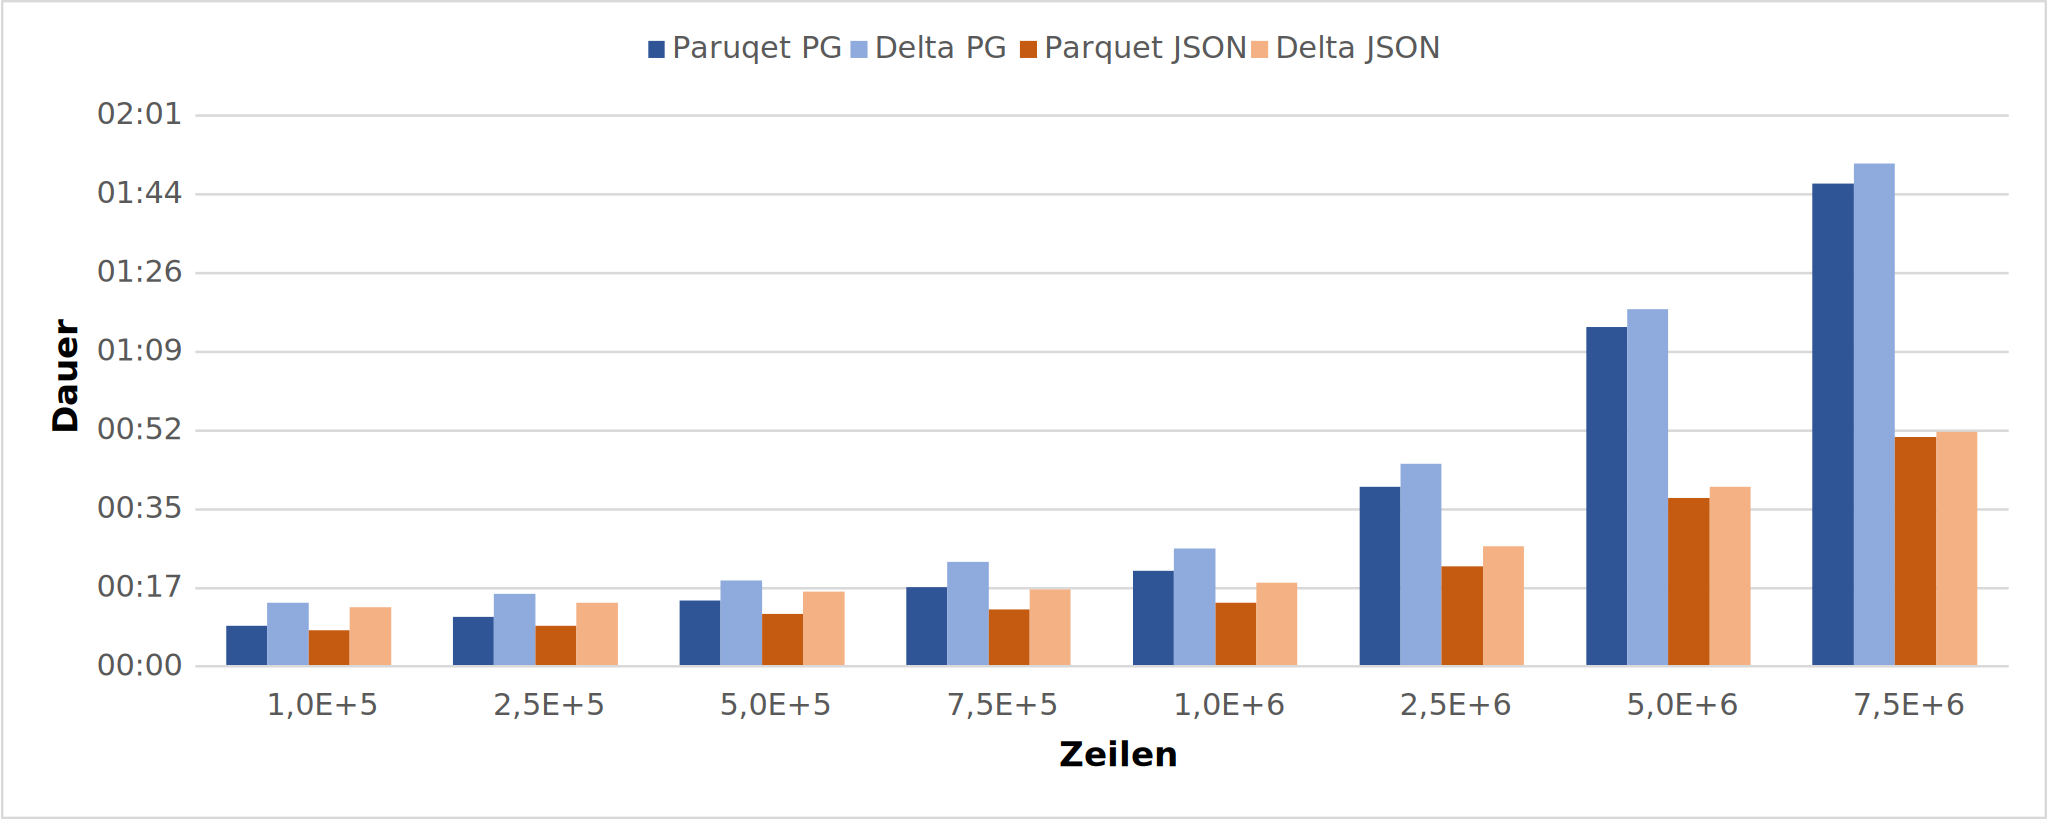
\includegraphics[width=\textwidth]{Grafiken/Evaluierung/Zeit-Initial}
    \label{fig:eval-time-i}
\end{figure}

\begin{figure}
    \centering
    \caption{Dauer Ingestion aus aktualisierten Daten}
    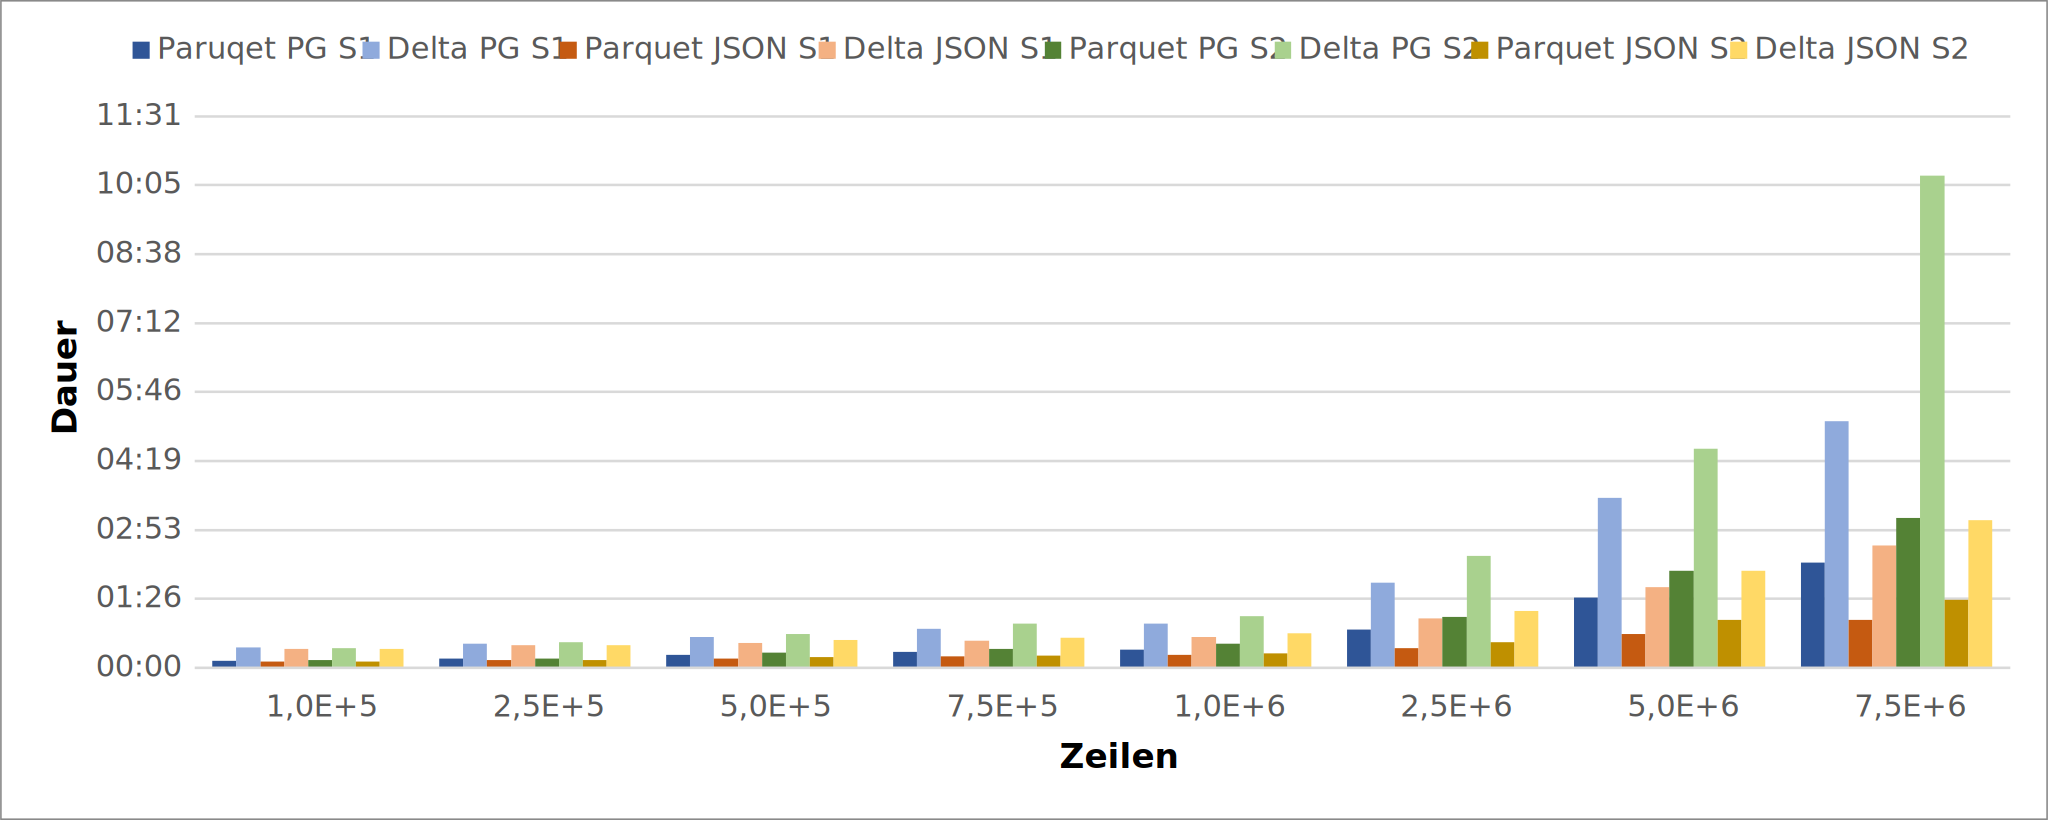
\includegraphics[width=\textwidth]{Grafiken/Evaluierung/Zeit-Update}
    \label{fig:eval-time-u}
\end{figure}

\begin{figure}
    \centering
    \caption{Dauer Ingestion aus Update-Quelle}
    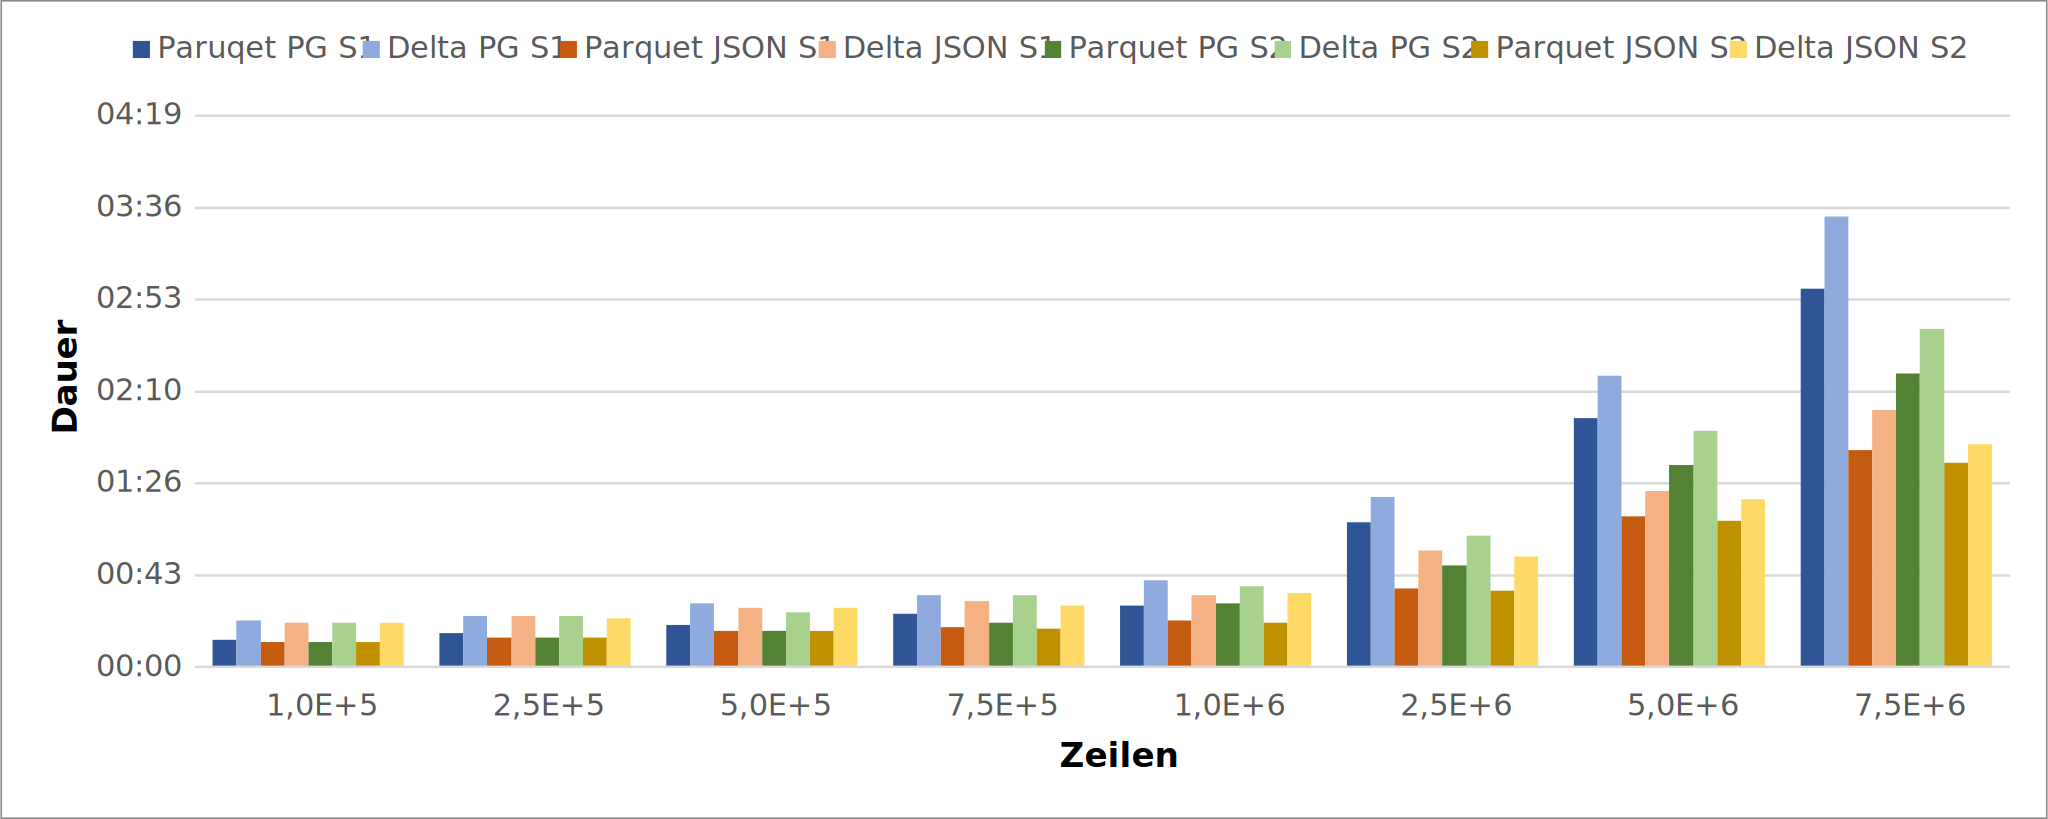
\includegraphics[width=\textwidth]{Grafiken/Evaluierung/Zeit-Cdc}
    \label{fig:eval-time-c}
\end{figure}

\subsubsection{Festplattenspeicherverbrauch}

Für die initiale Ingestion \cref{fig:eval-storage-i} ist kein Unterschied im Festplattenspeicherverbrauch zu erkennen.
Bei Betrachtung der genauen Werte ist zu sehen, dass die Delta-Tabellen einen leicht höheren Festplattenspeicherverbrauch haben.
Das liegt daran, dass Delta-Tabellen die Daten auch in Parquet speichern und nach der ersten Ingestion noch keine Versionierungsinformationen vorhanden sind.
Diese treten erst bei einer weiteren Ingestion auf.

Bei einer Ingestion von aktualisierten Daten (\cref{fig:eval-storage-u}) und aus einer Update-Quelle (\cref{fig:eval-storage-c}) ist der Festplattenspeicherverbrauch gleich.
Beide Quellen enthalten die gleichen Änderungen, weshalb auch das gespeicherte Ergebnis gleich sein muss.
Der Unterschied zwischen den Szenarien liegt darin, dass im zweiten Szenario mehr Daten eingefügt und weniger gelöscht werden, so dass am Ende mehr Daten im Datensatz enthalten sind.

Auch beim Festplattenspeicherverbrauch kommt die Eigenschaft der verschachtelten Daten in Spark zum Tragen.
Man sieht, dass weniger Spalteninformationen gespeichert werden müssen, was den Verbrauch niedriger hält.
Daraus lässt sich aber auch schließen, dass ohne weitere Verarbeitung weniger Informationen über Änderungen vorhanden sind.
Das heißt, dass bei Änderungen in einem verschachtelten Feld nur erkannt wird, dass sich das Feld auf der obersten Ebene darüber verändert hat.
Die genauen Änderungen müssen, durch zum Beispiel einen Vergleich der Versionen, nachträglich berechnet werden.


\begin{figure}
    \centering
    \caption{Festplattenspeicherverbrauch nach der ersten Ingestion}
    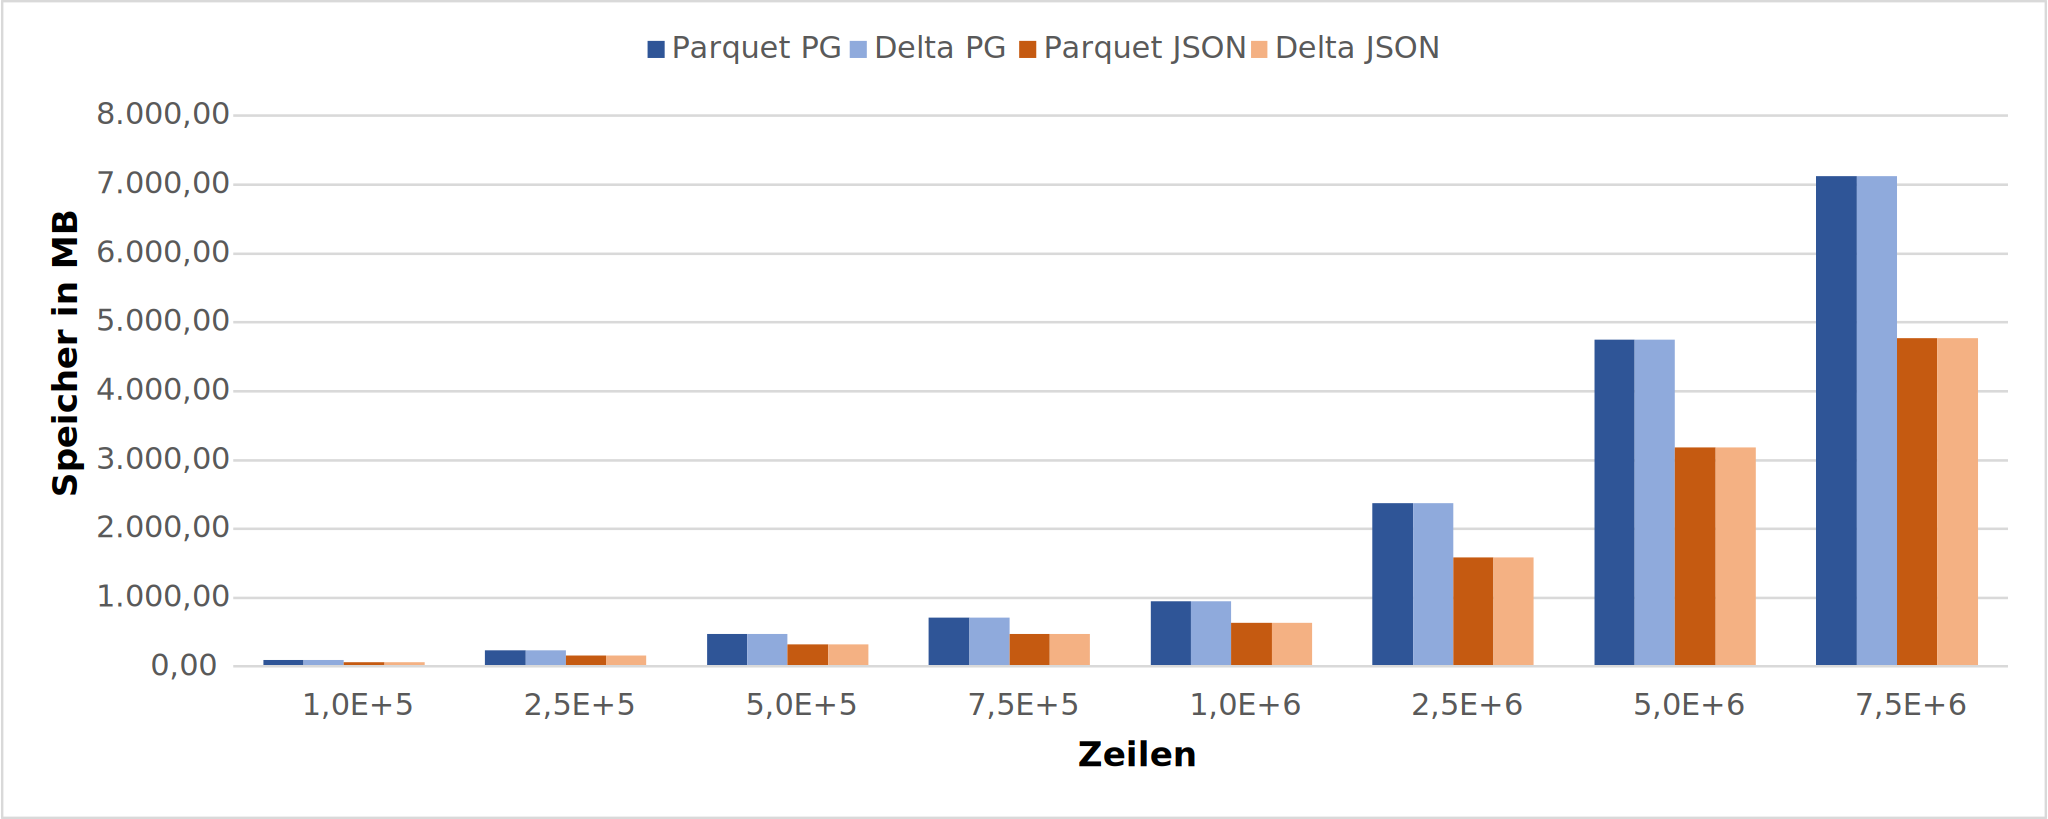
\includegraphics[width=\textwidth]{Grafiken/Evaluierung/Speicher-Initial}
    \label{fig:eval-storage-i}
\end{figure}

\begin{figure}
    \centering
    \caption{Festplattenspeicherverbrauch nach der Ingestion aus aktualisierten Daten}
    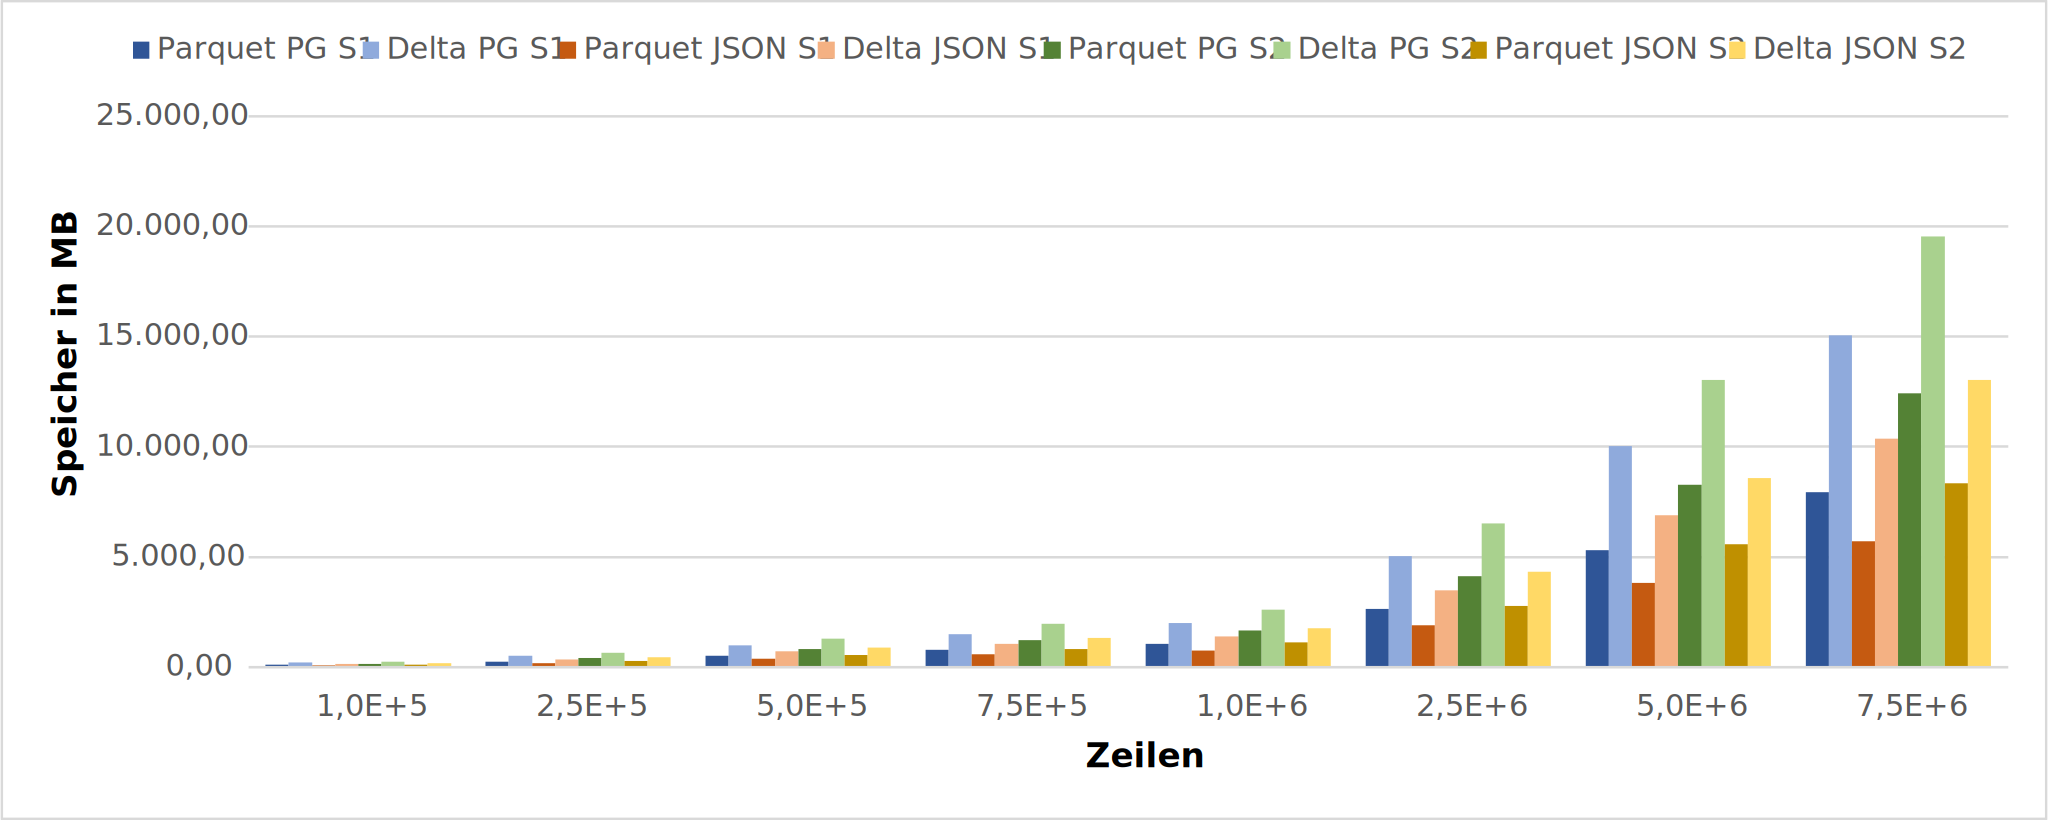
\includegraphics[width=\textwidth]{Grafiken/Evaluierung/Speicher-Update}
    \label{fig:eval-storage-u}
\end{figure}

\begin{figure}
    \centering
    \caption{Festplattenspeicherverbrauch nach der Ingestion aus Update-Quelle}
    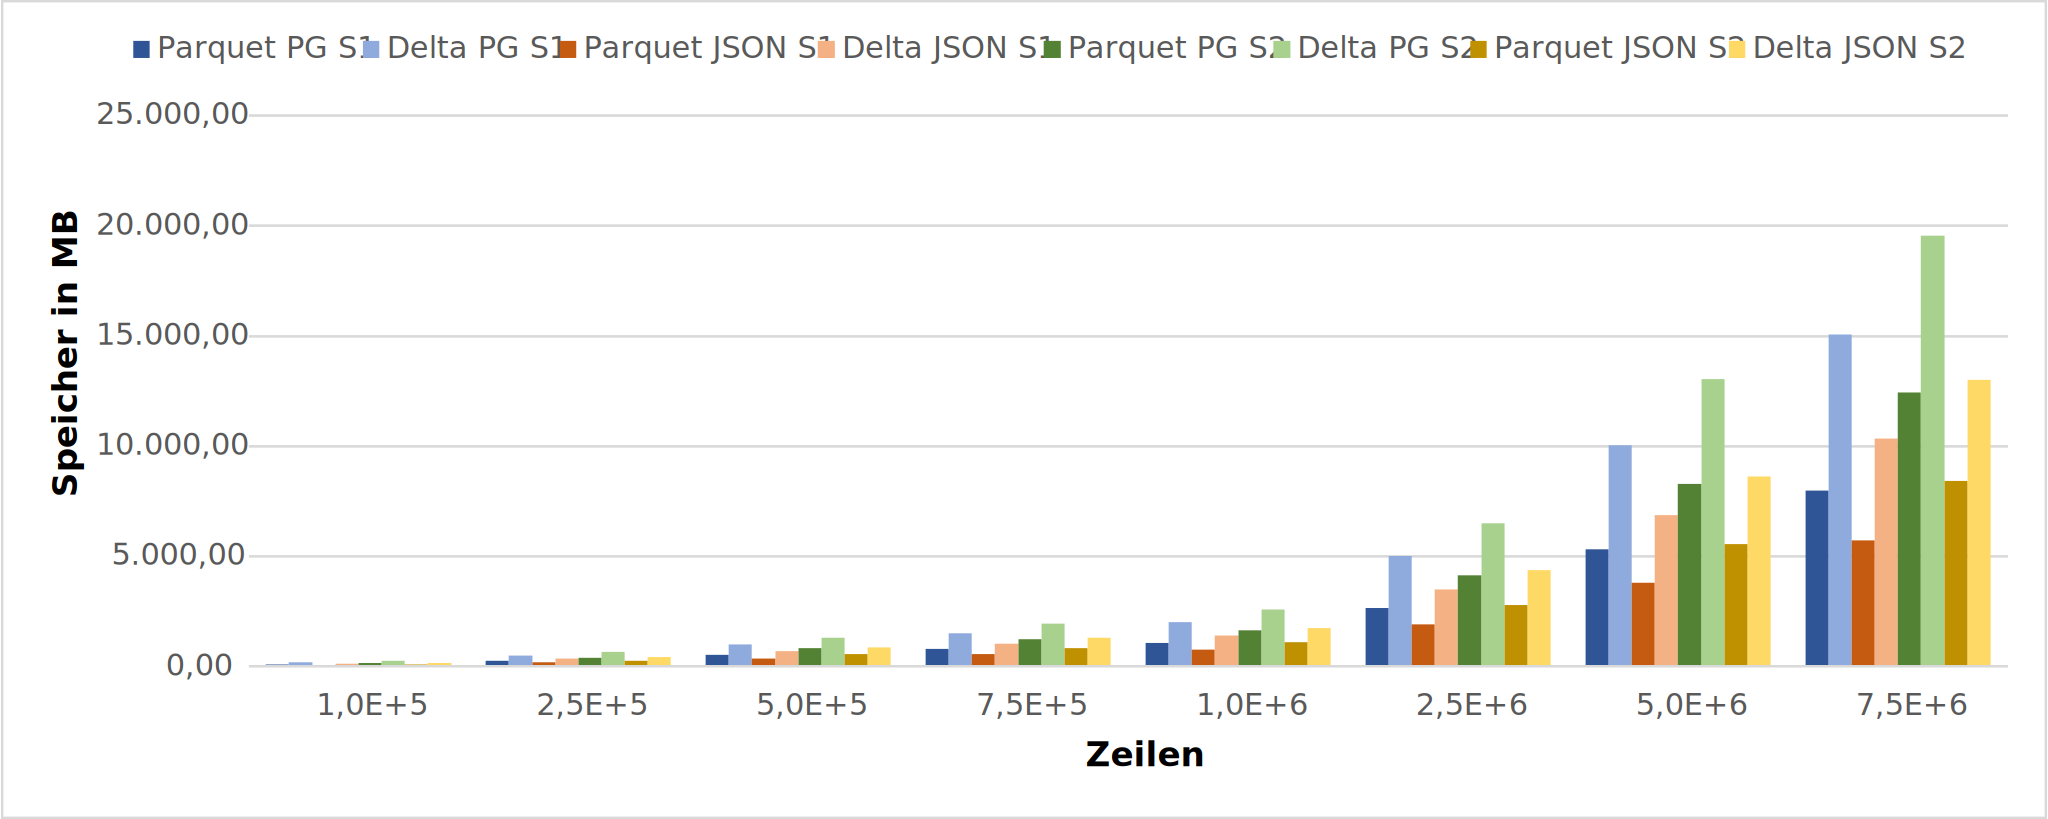
\includegraphics[width=\textwidth]{Grafiken/Evaluierung/Speicher-Cdc}
    \label{fig:eval-storage-c}
\end{figure}
\chapter{Zusammenfassung und Ausblick}

Die Aufgabenstellung dieser Arbeit war die Entwicklung einer Ingestion-Schnitt\-stelle für ein Data-Lake-System, dass im Kontext des HIT-Instituts an der Hochschule Niederrhein angewendet werden soll.
An diesem Institut werden Daten aus verschiedenen Quellen erfasst.
Es gibt klassische Datenbank-Systeme, Dateien oder REST-APIs.
Der Data Lake soll die zentrale Speicherlösung sein und Verarbeitungsprozesse unterstützen.
Dazu ist es neben der Unterstützung verschiedener Datenquellen auch nötig die Daten zu versioniern.
Dadurch verringert sich der Aufwand bei der weiteren Verarbeitung, da nur Änderungen betrachtet werden müssen.

In der vorliegenden Arbeit wurde eine generische Ingestion-Schnittstelle mit Versionierung für Data-Lake-Systeme entwickelt und mit funktionalen Tests und Benchmarks evaluiert.
Dafür wurde neben der Entwicklung der bestehende Prototyp des Data Lake auf eine Microservice-Archi\-tektur umgebaut.
Es wurden außerdem existierende Data-Lake-Systeme betrachtet und bewertet, ob diese als Lösung für die Problemstellung dienen könnten.
Daraus ergab sich, dass eine Eigenentwicklung notwendig ist.

Die Ingestion-Schnittstelle besteht aus drei Microservices.
Der Ingestion-Ser\-vice verwaltet das Laden von Daten in das System.
Dabei erlaubt die Verwendung von Spark und einem Plugin-System das Laden von Daten aus jeder Quelle.
Die kontinuierliche Ausführung von Ingestions wird durch den Continuation-Service sichergestellt.
Benutzer können über den API-Service mit der Ingestion-Schnittstelle interagieren.
Dieser besteht aus der Integration der neuen API in den Server des Prototyps.
Dadurch bleibt das System mit der Verwendung der alten API kompatibel.
Aus der Eingabe, die ein Benutzer an die API sendet, wird ein generelles Metadatenmodell aufgebaut.

Das Metadatenmodell zur Definition einer Datenquelle enthält alle Informationen über die Datenquelle, verwendete Plugins und zugehörige Ingestions.
Über dieses Modell werden die Informationen zu den Ingestions zwischen den Microservices ausgetauscht.

Neben der Ingestion-Schnittstelle besteht der Data Lake aus weiteren Komponenten.
Ein Kafka-Cluster wird für die Kommunikation im Data-Lake-System eingesetzt.
Diese kann auch für die Anbindung von Datenströmen verwendet werden.
Die Daten, die in den Data Lake geladen wurden, werden in einem HDFS gespeichert.
Daten mit Versionierung werden in einer Delta-Tabelle des Delta Lake abgelegt.
Für unversionierte Daten wird entweder das Parquet- oder, bei unstrukturierten Daten, das Ursprungsformat der Daten benutzt.
Für die Verwaltung von Metadaten kommt eine MongoDB-Datenbank zum Einsatz.
Die Datenverarbeitung geschieht über ein Spark-Cluster.

Die Evaluierung der Ingestion-Schnittstelle wurde in einem durch die gegebene Hardware möglichen Rahmen durchgeführt.
Hierfür stand kein leistungsstarkes Cluster zur Verfügung, um absolute Aussagen über die Leistung der Ingestion-Schnittstelle treffen zu können.
Daher ist lediglich ein relativer Vergleich ausgeführt worden, der Aussagen zur Skalierbarkeit des Ansatzes erlaubt.
Dabei wurden Benchmarks für verschiedene Datenmengen mit strukturierten und semistrukturierten Daten in zwei Szenarien ausgeführt.
Die Szenarien bilden dabei eine Situation, in der viele Änderungen an Daten geschehen und eine Situation, in der hauptsächlich Daten hinzugefügt werden ab.

Durch die Benchmarks und Tests wurde gezeigt, dass mit dieser Arbeit die Entwicklung der Ingestion-Schnittstelle noch nicht vollständig abgeschlossen ist.
Die implementierte Berechnung von Änderungsdaten ist in bestimmten Fällen sehr langsam.
Auch die Darstellung von Änderungen in verschachtelten Daten könnte durch ein anderes Vorgehen optimiert werden.
Somit ist die Versionierung in der Ingestion-Schnittstelle ein Thema, dass in einer anschließenden Arbeit genauer betrachtet werden kann.

Weiterhin sind die Metadaten, die während der Ingestion gesammelt werden, nicht ausreichend.
Um eine aussagekräftige Suche, Exploration und Analyse der Daten durchführen zu können, müssen direkt nach dem Laden weitere Metadaten automatisch extrahiert oder manuell durch einen Benutzer hinzugefügt werden.
Diese könnten zum Beispiel Informationen über den Inhalt oder die Struktur der Daten beinhalten.
Die in dieser Arbeit entwickelte Ingestion-Schnittstelle ist modular und erweiterbar aufgebaut, so dass in zukünftigen Arbeiten entsprechende Erweiterungen umgesetzt werden können.

\addcontentsline{toc}{chapter}{Abbildungsverzeichnis}
\listoffigures

\printbibliography
\addcontentsline{toc}{chapter}{Listeraturverzeichnis}

\appendix
\chapter{Benchmark Ergebnisse}
\label{sec:benchmark-tables}
Nachfolgend sind alle Ergebnisse der Benchmarks aufgelistet.
Zeiten sind dabei immer im Format Minuten:Sekunden.
In den Spaltenüberschriften werden die drei Buchstaben mit folgenden Bedeutungen verwendet:
\begin{description}
    \item[I]: Initiale Ingestion
    \item[U]: Ingestion mit aktualisierten Daten
    \item[C]: Ingestion mit Änderungsdaten
\end{description}

\begin{table}
    \centering
    \begin{tabular}{|r|r|r|r|r|r|r|}
        \hline
        \textbf{Zeilen} & \textbf{Speicher I} & \textbf{Zeit I} & \textbf{Speicher U} & \textbf{Zeit U} & \textbf{Speicher C} & \textbf{Zeit C} \\ \hline
        1,0e+3 & 0,96 MB       & 00:07 & 0,83 MB       & 00:07 & 0,84 MB       & 00:10 \\ \hline
        2,5e+3 & 2,39 MB       & 00:07 & 2,11 MB       & 00:07 & 2,11 MB       & 00:10 \\ \hline
        5,0e+3 & 4,75 MB       & 00:07 & 4,22 MB       & 00:07 & 4,22 MB       & 00:10 \\ \hline
        7,5e+3 & 7,12 MB       & 00:08 & 6,29 MB       & 00:08 & 6,30 MB       & 00:10 \\ \hline
        1,0e+4 & 9,48 MB       & 00:08 & 8,47 MB       & 00:08 & 8,47 MB       & 00:10 \\ \hline
        2,5e+4 & 23,66 MB      & 00:08 & 21,14 MB      & 00:08 & 24,45 MB      & 00:10 \\ \hline
        5,0e+4 & 47,30 MB      & 00:09 & 52,77 MB      & 00:08 & 52,30 MB      & 00:11 \\ \hline
        7,5e+4 & 70,94 MB      & 00:09 & 79,15 MB      & 00:09 & 79,23 MB      & 00:12 \\ \hline
        1,0e+5 & 94,57 MB      & 00:09 & 105,38 MB     & 00:09 & 105,70 MB     & 00:13 \\ \hline
        2,5e+5 & 236,39 MB     & 00:11 & 264,49 MB     & 00:12 & 264,71 MB     & 00:16 \\ \hline
        5,0e+5 & 474,70 MB     & 00:15 & 531,68 MB     & 00:16 & 529,78 MB     & 00:20 \\ \hline
        7,5e+5 & 711,06 MB     & 00:18 & 796,23 MB     & 00:20 & 795,45 MB     & 00:25 \\ \hline
        1,0e+6 & 949,38 MB     & 00:21 & 1.060,58 MB   & 00:23 & 1.060,46 MB   & 00:29 \\ \hline
        2,5e+6 & 2.373,41 MB   & 00:40 & 2.651,87 MB   & 00:48 & 2.657,99 MB   & 01:08 \\ \hline
        5,0e+6 & 4.748,75 MB   & 01:16 & 5.305,38 MB   & 01:28 & 5.318,29 MB   & 01:57 \\ \hline
        7,5e+6 & 7.124,09 MB   & 01:47 & 7.956,28 MB   & 02:12 & 7.977,94 MB   & 02:58 \\ \hline

    \end{tabular}
    \caption{Strukturierte Daten - Fall 1 - Ohne Versionierung}
\end{table}

\begin{table}
    \centering
    \begin{tabular}{|r|r|r|r|r|r|r|}
        \hline
        \textbf{Zeilen} & \textbf{Speicher I} & \textbf{Zeit I} & \textbf{Speicher U} & \textbf{Zeit U} & \textbf{Speicher C} & \textbf{Zeit C} \\ \hline
        1,0e+3  & 0,96 MB       & 00:13 & 4,19 MB       & 00:22 & 4,19 MB       & 00:20 \\ \hline
        2,5e+3  & 2,39 MB       & 00:13 & 7,22 MB       & 00:22 & 7,22 MB       & 00:20 \\ \hline
        5,0e+3  & 4,76 MB       & 00:13 & 12,28 MB      & 00:23 & 12,28 MB      & 00:20 \\ \hline
        7,5e+3  & 7,12 MB       & 00:13 & 17,32 MB      & 00:23 & 17,32 MB      & 00:21 \\ \hline
        1,0e+4  & 9,48 MB       & 00:14 & 22,35 MB      & 00:22 & 22,35 MB      & 00:20 \\ \hline
        2,5e+4  & 23,67 MB      & 00:13 & 52,49 MB      & 00:23 & 52,49 MB      & 00:20 \\ \hline
        5,0e+4  & 47,30 MB      & 00:13 & 102,70 MB     & 00:23 & 102,70 MB     & 00:21 \\ \hline
        7,5e+4  & 70,94 MB      & 00:13 & 152,90 MB     & 00:25 & 152,90 MB     & 00:21 \\ \hline
        1,0e+5  & 94,57 MB      & 00:14 & 203,10 MB     & 00:26 & 203,10 MB     & 00:22 \\ \hline
        2,5e+5  & 236,39 MB     & 00:16 & 504,28 MB     & 00:30 & 504,28 MB     & 00:24 \\ \hline
        5,0e+5  & 474,70 MB     & 00:19 & 1.008,09 MB   & 00:39 & 1.008,09 MB   & 00:30 \\ \hline
        7,5e+5  & 711,06 MB     & 00:23 & 1.509,56 MB   & 00:49 & 1.509,56 MB   & 00:34 \\ \hline
        1,0e+6 & 949,38 MB     & 00:26 & 2.012,54 MB   & 00:55 & 2.012,54 MB   & 00:41 \\ \hline
        2,5e+6 & 2.373,41 MB   & 00:45 & 5.024,57 MB   & 01:47 & 5.024,57 MB   & 01:20 \\ \hline
        5,0e+6 & 4.748,75 MB   & 01:18 & 10.046,59 MB  & 03:33 & 10.046,59 MB  & 02:17 \\ \hline
        7,5e+6 & 7.124,09 MB   & 01:51 & 15.058,13 MB  & 05:09 & 15.058,13 MB  & 03:32 \\ \hline
    \end{tabular}
    \caption{Strukturierte Daten - Fall 1 - Mit Versionierung}
\end{table}

\begin{table}
    \centering
    \begin{tabular}{|r|r|r|r|r|r|r|}
        \hline
        \textbf{Zeilen} & \textbf{Speicher I} & \textbf{Zeit I} & \textbf{Speicher U} & \textbf{Zeit U} & \textbf{Speicher C} & \textbf{Zeit C} \\ \hline
        1,0e+3 & 0,65 MB       & 00:08 & 7,94 MB       & 00:07 & 7,82 MB       & 00:10 \\ \hline
        2,5e+3 & 1,61 MB       & 00:07 & 19,50 MB      & 00:07 & 19,34 MB      & 00:10 \\ \hline
        5,0e+3 & 3,21 MB       & 00:07 & 38,67 MB      & 00:07 & 38,42 MB      & 00:11 \\ \hline
        7,5e+3 & 4,80 MB       & 00:08 & 57,79 MB      & 00:07 & 57,50 MB      & 00:10 \\ \hline
        1,0e+4 & 6,39 MB       & 00:08 & 76,87 MB      & 00:07 & 76,58 MB      & 00:10 \\ \hline
        2,5e+4 & 15,92 MB      & 00:08 & 191,32 MB     & 00:07 & 191,43 MB     & 00:11 \\ \hline
        5,0e+4 & 31,81 MB      & 00:08 & 382,01 MB     & 00:07 & 382,95 MB     & 00:11 \\ \hline
        7,5e+4 & 47,73 MB      & 00:08 & 573,05 MB     & 00:07 & 573,80 MB     & 00:12 \\ \hline
        1,0e+5 & 63,63 MB      & 00:08 & 763,73 MB     & 00:08 & 766,76 MB     & 00:12 \\ \hline
        2,5e+5 & 159,07 MB     & 00:09 & 1.909,18 MB   & 00:10 & 1.915,76 MB   & 00:14 \\ \hline
        5,0e+5 & 318,15 MB     & 00:12 & 3.818,39 MB   & 00:12 & 3.832,67 MB   & 00:17 \\ \hline
        7,5e+5 & 477,25 MB     & 00:13 & 5.727,59 MB   & 00:14 & 5.738,92 MB   & 00:19 \\ \hline
        1,0e+6 & 636,31 MB     & 00:15 & 7.636,83 MB   & 00:16 & 7.645,30 MB   & 00:22 \\ \hline
        2,5e+6 & 1.590,86 MB   & 00:22 & 19.092,19 MB  & 00:25 & 19.023,51 MB  & 00:37 \\ \hline
        5,0e+6 & 3.181,51 MB   & 00:35 & 38.183,02 MB  & 00:42 & 38.129,25 MB  & 01:11 \\ \hline
        7,5e+6 & 4.772,36 MB   & 00:49 & 57.275,36 MB  & 01:00 & 57.418,35 MB  & 01:42 \\ \hline
    \end{tabular}
    \caption{Semistrukturierte Daten - Fall 1 - Ohne Versionierung}
\end{table}

\begin{table}
    \centering
    \begin{tabular}{|r|r|r|r|r|r|r|}
        \hline
        \textbf{Zeilen} & \textbf{Speicher I} & \textbf{Zeit I} & \textbf{Speicher U} & \textbf{Zeit U} & \textbf{Speicher C} & \textbf{Zeit C} \\ \hline
        1,0e+3 & 0,65 MB        & 00:14 & 3,28 MB       & 00:23 & 3,28 MB       & 00:19 \\ \hline
        2,5e+3 & 1,61 MB        & 00:12 & 5,43 MB       & 00:21 & 5,43 MB       & 00:20 \\ \hline
        5,0e+3 & 3,21 MB        & 00:13 & 9,00 MB       & 00:22 & 9,00 MB       & 00:20 \\ \hline
        7,5e+3 & 4,80 MB        & 00:12 & 12,56 MB      & 00:21 & 12,56 MB      & 00:19 \\ \hline
        1,0e+4 & 6,39 MB        & 00:13 & 16,09 MB      & 00:22 & 16,10 MB      & 00:20 \\ \hline
        2,5e+4 & 15,92 MB       & 00:13 & 37,27 MB      & 00:23 & 37,28 MB      & 00:20 \\ \hline
        5,0e+4 & 31,81 MB       & 00:13 & 72,58 MB      & 00:24 & 72,60 MB      & 00:21 \\ \hline
        7,5e+4 & 47,74 MB       & 00:13 & 107,90 MB     & 00:24 & 107,99 MB     & 00:21 \\ \hline
        1,0e+5 & 63,63 MB       & 00:13 & 143,32 MB     & 00:24 & 143,32 MB     & 00:21 \\ \hline
        2,5e+5 & 159,08 MB      & 00:14 & 354,70 MB     & 00:28 & 354,70 MB     & 00:24 \\ \hline
        5,0e+5 & 318,16 MB      & 00:16 & 706,04 MB     & 00:31 & 706,05 MB     & 00:28 \\ \hline
        7,5e+5 & 477,25 MB      & 00:17 & 1.055,49 MB   & 00:34 & 1.055,50 MB   & 00:31 \\ \hline
        1,0e+6 & 636,32 MB      & 00:19 & 1.404,25 MB   & 00:39 & 1.404,25 MB   & 00:34 \\ \hline
        2,5e+6 & 1.590,87 MB    & 00:27 & 3.496,49 MB   & 01:02 & 3.498,78 MB   & 00:55 \\ \hline
        5,0e+6 & 3.181,53 MB    & 00:39 & 6.900,47 MB   & 01:41 & 6.888,11 MB   & 01:23 \\ \hline
        7,5e+6 & 4.772,39 MB    & 00:53 & 10.359,32 MB  & 02:33 & 10.361,91 MB  & 02:01 \\ \hline
    \end{tabular}
    \caption{Semistrukturierte Daten - Fall 1 - Mit Versionierung}
\end{table}

\begin{table}
    \centering
    \begin{tabular}{|r|r|r|r|r|r|r|}
        \hline
        \textbf{Zeilen} & \textbf{Speicher I} & \textbf{Zeit I} & \textbf{Speicher U} & \textbf{Zeit U} & \textbf{Speicher C} & \textbf{Zeit C} \\ \hline
        1,0e+3  & 0,96 MB       & 00:07 & 1,02 MB       & 00:07 & 1,02 MB       & 00:10 \\ \hline
        2,5e+3  & 2,39 MB       & 00:07 & 2,57 MB       & 00:07 & 2,57 MB       & 00:10 \\ \hline
        5,0e+3  & 4,75 MB       & 00:07 & 5,15 MB       & 00:07 & 5,15 MB       & 00:09 \\ \hline
        7,5e+3  & 7,12 MB       & 00:08 & 7,71 MB       & 00:08 & 7,71 MB       & 00:10 \\ \hline
        1,0e+4  & 9,48 MB       & 00:07 & 10,33 MB      & 00:07 & 10,33 MB      & 00:10 \\ \hline
        2,5e+4  & 23,66 MB      & 00:08 & 25,94 MB      & 00:08 & 34,81 MB      & 00:11 \\ \hline
        5,0e+4  & 47,30 MB      & 00:08 & 82,51 MB      & 00:09 & 78,24 MB      & 00:11 \\ \hline
        7,5e+4  & 70,94 MB      & 00:09 & 123,75 MB     & 00:09 & 122,05 MB     & 00:12 \\ \hline
        1,0e+5  & 94,57 MB      & 00:09 & 164,99 MB     & 00:10 & 162,62 MB     & 00:12 \\ \hline
        2,5e+5  & 236,39 MB     & 00:11 & 414,83 MB     & 00:12 & 413,71 MB     & 00:14 \\ \hline
        5,0e+5  & 474,70 MB     & 00:14 & 827,02 MB     & 00:19 & 827,06 MB     & 00:17 \\ \hline
        7,5e+5  & 711,06 MB     & 00:17 & 1.240,49 MB   & 00:24 & 1.240,20 MB   & 00:21 \\ \hline
        1,0e+6  & 949,38 MB     & 00:21 & 1.658,10 MB   & 00:30 & 1.653,52 MB   & 00:30 \\ \hline
        2,5e+6  & 2.373,41 MB   & 00:39 & 4.142,78 MB   & 01:04 & 4.136,67 MB   & 00:48 \\ \hline
        5,0e+6  & 4.748,75 MB   & 01:13 & 8.284,29 MB   & 02:02 & 8.276,20 MB   & 01:35 \\ \hline
        7,5e+6  & 7.124,09 MB   & 01:45 & 12.430,15 MB  & 03:08 & 12.458,08 MB  & 02:18 \\ \hline
    \end{tabular}
    \caption{Strukturierte Daten - Fall 2 - Ohne Versionierung}
\end{table}

\begin{table}
    \centering
    \begin{tabular}{|r|r|r|r|r|r|r|}
        \hline
        \textbf{Zeilen} & \textbf{Speicher I} & \textbf{Zeit I} & \textbf{Speicher U} & \textbf{Zeit U} & \textbf{Speicher C} & \textbf{Zeit C} \\ \hline
        1,0e+3  & 0,96 MB       & 00:14 & 4,75 MB       & 00:21 & 4,75 MB       & 00:19 \\ \hline
        2,5e+3  & 2,39 MB       & 00:12 & 8,72 MB       & 00:21 & 8,72 MB       & 00:18 \\ \hline
        5,0e+3  & 4,76 MB       & 00:13 & 15,29 MB      & 00:22 & 15,29 MB      & 00:19 \\ \hline
        7,5e+3  & 7,12 MB       & 00:13 & 21,82 MB      & 00:22 & 21,82 MB      & 00:19 \\ \hline
        1,0e+4  & 9,48 MB       & 00:12 & 28,36 MB      & 00:20 & 28,36 MB      & 00:19 \\ \hline
        2,5e+4  & 23,67 MB      & 00:13 & 67,52 MB      & 00:22 & 67,52 MB      & 00:19 \\ \hline
        5,0e+4  & 47,30 MB      & 00:14 & 132,74 MB     & 00:24 & 132,74 MB     & 00:21 \\ \hline
        7,5e+4  & 70,94 MB      & 00:14 & 197,88 MB     & 00:25 & 197,88 MB     & 00:21 \\ \hline
        1,0e+5  & 94,57 MB      & 00:14 & 263,10 MB     & 00:25 & 263,10 MB     & 00:21 \\ \hline
        2,5e+5  & 236,39 MB     & 00:16 & 654,40 MB     & 00:32 & 654,40 MB     & 00:24 \\ \hline
        5,0e+5  & 474,70 MB     & 00:19 & 1.307,04 MB   & 00:42 & 1.307,04 MB   & 00:26 \\ \hline
        7,5e+5  & 711,06 MB     & 00:23 & 1.956,73 MB   & 00:55 & 1.956,73 MB   & 00:34 \\ \hline
        1,0e+6  & 949,38 MB     & 00:26 & 2.608,57 MB   & 01:05 & 2.608,57 MB   & 00:38 \\ \hline
        2,5e+6  & 2.373,41 MB   & 00:44 & 6.512,17 MB   & 02:20 & 6.512,17 MB   & 01:02 \\ \hline
        5,0e+6  & 4.748,75 MB   & 01:19 & 13.035,43 MB  & 04:35 & 13.035,43 MB  & 01:51 \\ \hline
        7,5e+6  & 7.124,09 MB   & 01:50 & 19.542,27 MB  & 10:17 & 19.542,27 MB  & 02:39 \\ \hline
    \end{tabular}
    \caption{Strukturierte Daten - Fall 2 - Mit Versionierung}
\end{table}

\begin{table}
    \centering
    \begin{tabular}{|r|r|r|r|r|r|r|}
        \hline
        \textbf{Zeilen} & \textbf{Speicher I} & \textbf{Zeit I} & \textbf{Speicher U} & \textbf{Zeit U} & \textbf{Speicher C} & \textbf{Zeit C} \\ \hline
        1,0e+3  & 0,65 MB       & 00:10 & 1,14 MB       & 00:07 & 1,13 MB       & 00:10 \\ \hline
        2,5e+3  & 1,61 MB       & 00:07 & 2,83 MB       & 00:07 & 2,80 MB       & 00:10 \\ \hline
        5,0e+3  & 3,21 MB       & 00:07 & 5,62 MB       & 00:07 & 5,58 MB       & 00:11 \\ \hline
        7,5e+3  & 4,80 MB       & 00:07 & 8,40 MB       & 00:07 & 8,36 MB       & 00:10 \\ \hline
        1,0e+4  & 6,39 MB       & 00:07 & 11,18 MB      & 00:07 & 11,15 MB      & 00:10 \\ \hline
        2,5e+4  & 15,92 MB      & 00:07 & 27,87 MB      & 00:08 & 27,89 MB      & 00:11 \\ \hline
        5,0e+4  & 31,81 MB      & 00:08 & 55,68 MB      & 00:08 & 55,83 MB      & 00:11 \\ \hline
        7,5e+4  & 47,73 MB      & 00:08 & 83,55 MB      & 00:08 & 83,61 MB      & 00:11 \\ \hline
        1,0e+5  & 63,63 MB      & 00:08 & 111,36 MB     & 00:08 & 111,65 MB     & 00:12 \\ \hline
        2,5e+5  & 159,07 MB     & 00:09 & 278,39 MB     & 00:10 & 279,37 MB     & 00:14 \\ \hline
        5,0e+5  & 318,15 MB     & 00:11 & 556,80 MB     & 00:13 & 558,88 MB     & 00:17 \\ \hline
        7,5e+5  & 477,25 MB     & 00:12 & 835,20 MB     & 00:15 & 837,07 MB     & 00:18 \\ \hline
        1,0e+6  & 636,31 MB     & 00:13 & 1.113,59 MB   & 00:18 & 1.115,78 MB   & 00:21 \\ \hline
        2,5e+6  & 1.590,86 MB   & 00:22 & 2.784,02 MB   & 00:32 & 2.781,98 MB   & 00:36 \\ \hline
        5,0e+6  & 3.181,51 MB   & 00:39 & 5.567,79 MB   & 01:00 & 5.576,58 MB   & 01:09 \\ \hline
        7,5e+6  & 4.772,36 MB   & 00:52 & 8.351,79 MB   & 01:25 & 8.412,88 MB   & 01:36 \\ \hline
    \end{tabular}
    \caption{Semistrukturierte Daten - Fall 2 - Ohne Versionierung}
\end{table}

\begin{table}
    \centering
    \begin{tabular}{|r|r|r|r|r|r|r|}
        \hline
        \textbf{Zeilen} & \textbf{Speicher I} & \textbf{Zeit I} & \textbf{Speicher U} & \textbf{Zeit U} & \textbf{Speicher C} & \textbf{Zeit C} \\ \hline
        1,0e+3  & 0,65 MB       & 00:15 & 3,64 MB       & 00:22 & 3,64 MB       & 00:19 \\ \hline
        2,5e+3  & 1,61 MB       & 00:12 & 6,34 MB       & 00:21 & 6,34 MB       & 00:20 \\ \hline
        5,0e+3  & 3,21 MB       & 00:12 & 10,80 MB      & 00:22 & 10,80 MB      & 00:19 \\ \hline
        7,5e+3  & 4,80 MB       & 00:13 & 15,23 MB      & 00:23 & 15,24 MB      & 00:20 \\ \hline
        1,0e+4  & 6,39 MB       & 00:12 & 19,65 MB      & 00:22 & 19,67 MB      & 00:19 \\ \hline
        2,5e+4  & 15,92 MB      & 00:13 & 46,13 MB      & 00:22 & 46,18 MB      & 00:20 \\ \hline
        5,0e+4  & 31,81 MB      & 00:13 & 90,38 MB      & 00:24 & 90,49 MB      & 00:21 \\ \hline
        7,5e+4  & 47,74 MB      & 00:13 & 134,39 MB     & 00:24 & 134,62 MB     & 00:21 \\ \hline
        1,0e+5  & 63,63 MB      & 00:13 & 178,73 MB     & 00:24 & 178,73 MB     & 00:21 \\ \hline
        2,5e+5  & 159,08 MB     & 00:14 & 443,04 MB     & 00:28 & 443,05 MB     & 00:23 \\ \hline
        5,0e+5  & 318,16 MB     & 00:17 & 881,61 MB     & 00:35 & 881,76 MB     & 00:28 \\ \hline
        7,5e+5  & 477,25 MB     & 00:17 & 1.316,34 MB   & 00:38 & 1.316,35 MB   & 00:29 \\ \hline
        1,0e+6  & 636,32 MB     & 00:18 & 1.752,75 MB   & 00:43 & 1.754,19 MB   & 00:35 \\ \hline
        2,5e+6  & 1.590,87 MB   & 00:26 & 4.343,15 MB   & 01:11 & 4.377,65 MB   & 00:52 \\ \hline
        5,0e+6  & 3.181,53 MB   & 00:40 & 8.573,33 MB   & 02:02 & 8.637,57 MB   & 01:19 \\ \hline
        7,5e+6  & 4.772,39 MB   & 00:50 & 13.028,96 MB  & 03:05 & 13.029,04 MB  & 01:45 \\ \hline
    \end{tabular}
    \caption{Semistrukturierte Daten - Fall 2 - Mit Versionierung}
\end{table}


















\end{document}
